% Options for packages loaded elsewhere
\PassOptionsToPackage{unicode}{hyperref}
\PassOptionsToPackage{hyphens}{url}
%
\documentclass[
]{book}
\usepackage{amsmath,amssymb}
\usepackage{iftex}
\ifPDFTeX
  \usepackage[T1]{fontenc}
  \usepackage[utf8]{inputenc}
  \usepackage{textcomp} % provide euro and other symbols
\else % if luatex or xetex
  \usepackage{unicode-math} % this also loads fontspec
  \defaultfontfeatures{Scale=MatchLowercase}
  \defaultfontfeatures[\rmfamily]{Ligatures=TeX,Scale=1}
\fi
\usepackage{lmodern}
\ifPDFTeX\else
  % xetex/luatex font selection
\fi
% Use upquote if available, for straight quotes in verbatim environments
\IfFileExists{upquote.sty}{\usepackage{upquote}}{}
\IfFileExists{microtype.sty}{% use microtype if available
  \usepackage[]{microtype}
  \UseMicrotypeSet[protrusion]{basicmath} % disable protrusion for tt fonts
}{}
\makeatletter
\@ifundefined{KOMAClassName}{% if non-KOMA class
  \IfFileExists{parskip.sty}{%
    \usepackage{parskip}
  }{% else
    \setlength{\parindent}{0pt}
    \setlength{\parskip}{6pt plus 2pt minus 1pt}}
}{% if KOMA class
  \KOMAoptions{parskip=half}}
\makeatother
\usepackage{xcolor}
\usepackage{longtable,booktabs,array}
\usepackage{calc} % for calculating minipage widths
% Correct order of tables after \paragraph or \subparagraph
\usepackage{etoolbox}
\makeatletter
\patchcmd\longtable{\par}{\if@noskipsec\mbox{}\fi\par}{}{}
\makeatother
% Allow footnotes in longtable head/foot
\IfFileExists{footnotehyper.sty}{\usepackage{footnotehyper}}{\usepackage{footnote}}
\makesavenoteenv{longtable}
\usepackage{graphicx}
\makeatletter
\newsavebox\pandoc@box
\newcommand*\pandocbounded[1]{% scales image to fit in text height/width
  \sbox\pandoc@box{#1}%
  \Gscale@div\@tempa{\textheight}{\dimexpr\ht\pandoc@box+\dp\pandoc@box\relax}%
  \Gscale@div\@tempb{\linewidth}{\wd\pandoc@box}%
  \ifdim\@tempb\p@<\@tempa\p@\let\@tempa\@tempb\fi% select the smaller of both
  \ifdim\@tempa\p@<\p@\scalebox{\@tempa}{\usebox\pandoc@box}%
  \else\usebox{\pandoc@box}%
  \fi%
}
% Set default figure placement to htbp
\def\fps@figure{htbp}
\makeatother
\setlength{\emergencystretch}{3em} % prevent overfull lines
\providecommand{\tightlist}{%
  \setlength{\itemsep}{0pt}\setlength{\parskip}{0pt}}
\setcounter{secnumdepth}{5}
\usepackage{booktabs}
\usepackage[]{natbib}
\bibliographystyle{plainnat}
\usepackage{bookmark}
\IfFileExists{xurl.sty}{\usepackage{xurl}}{} % add URL line breaks if available
\urlstyle{same}
\hypersetup{
  pdftitle={Mathematical Logic},
  pdfauthor={Ashan De Silva},
  hidelinks,
  pdfcreator={LaTeX via pandoc}}

\title{Mathematical Logic}
\author{Ashan De Silva}
\date{2025-08-19}

\usepackage{amsthm}
\newtheorem{theorem}{Theorem}[chapter]
\newtheorem{lemma}{Lemma}[chapter]
\newtheorem{corollary}{Corollary}[chapter]
\newtheorem{proposition}{Proposition}[chapter]
\newtheorem{conjecture}{Conjecture}[chapter]
\theoremstyle{definition}
\newtheorem{definition}{Definition}[chapter]
\theoremstyle{definition}
\newtheorem{example}{Example}[chapter]
\theoremstyle{definition}
\newtheorem{exercise}{Exercise}[chapter]
\theoremstyle{definition}
\newtheorem{hypothesis}{Hypothesis}[chapter]
\theoremstyle{remark}
\newtheorem*{remark}{Remark}
\newtheorem*{solution}{Solution}
\begin{document}
\maketitle

{
\setcounter{tocdepth}{1}
\tableofcontents
}
\chapter{Introduction}\label{introduction}

Mathematical logic is the discipline that formalizes reasoning. It provides a rigorous framework for analyzing statements, constructing arguments, and establishing truth. This textbook is designed to guide students through the foundational principles of logic, beginning with propositional logic and progressing toward predicate logic, proof techniques, and the structure of the real number system.

The study of logic is essential for all areas of mathematics. It enables us to distinguish valid reasoning from fallacy, to express mathematical ideas with precision, and to construct proofs that are both sound and complete. Logic also serves as a bridge between mathematics and computer science, philosophy, and linguistics, where formal reasoning plays a central role.

This book is structured to support both conceptual understanding and technical mastery. Each chapter introduces key definitions, examples, and formal notation, followed by exercises that reinforce the material. The progression is cumulative: later chapters build upon the logical foundations established early on.

\begin{center}\rule{0.5\linewidth}{0.5pt}\end{center}

\section{Chapter Overview}\label{chapter-overview}

\begin{itemize}
\item
  \textbf{Chapter 2: Mathematical Logic}\\
  Introduces propositional and predicate logic, truth tables, logical equivalence, and the algebra of propositions.
\item
  \textbf{Chapter 3: Introduction to Proofs}\\
  Covers terminology, argument structure, validity, and various proof techniques including indirect proofs and proof by cases.
\item
  \textbf{Chapter 4: The Real Number System ℝ}\\
  Presents the axioms of real numbers, properties of equality, order, completeness, and the concept of infinity.
\item
  \textbf{Chapter 5: Set Theory}\\
  Introduces the language of sets, operations, and foundational concepts used throughout mathematics.
\item
  \textbf{Chapter 6: Exercises}\\
  Provides practice problems to reinforce the concepts and techniques introduced in earlier chapters.
\end{itemize}

\begin{center}\rule{0.5\linewidth}{0.5pt}\end{center}

This textbook reflects a commitment to clarity, rigor, and accessibility. It is intended for undergraduate students beginning their study of mathematical logic, and for anyone seeking a structured and principled approach to formal reasoning.

\chapter{Mathematical logic}\label{mathematical-logic}

Mathematical logic is the branch of mathematics that studies the principles and methods of formal reasoning. It is based on symbolic languages that can express statements and arguments in a precise and unambiguous way.

\section{Propositional logic \& Logical operators}\label{propositional-logic-logical-operators}

Propositional logic is a branch of mathematical logic that studies the logical relationships between propositions, which are statements that can be either true or false.

\begin{definition}[Proposition (Statement)]
\protect\hypertarget{def:unnamed-chunk-1}{}\label{def:unnamed-chunk-1}Proposition (Statement) is a declarative sentence that is either true (T) or false (F), but not both.
\end{definition}

\begin{example}
\protect\hypertarget{exm:unnamed-chunk-2}{}\label{exm:unnamed-chunk-2}\leavevmode

\begin{enumerate}
\def\labelenumi{(\roman{enumi})}
\tightlist
\item
  A square has all its sides equal.
\item
  Every Odd number is not divisible by 2.
\item
  \(2 < 3\).
\item
  \(\sqrt{2}\not\in \mathbb{Q}\).
\item
  \(\mathbb{Z}\subseteq \mathbb{Q}\).
\item
  The set \(\{10, 20, 30\}\) has three elements.
\end{enumerate}

They are all true.

\end{example}

\begin{example}
\protect\hypertarget{exm:unnamed-chunk-3}{}\label{exm:unnamed-chunk-3}\leavevmode

\begin{enumerate}
\def\labelenumi{(\roman{enumi})}
\tightlist
\item
  Every rectangle is a square.
\item
  \((2 +4)^2 = 2^2 4^2\).
\item
  \(\sqrt{2}\not\in\mathbb{R}\).
\item
  \(\mathbb{R} \subseteq \mathbb{Q}\).
\item
  \(\{10, 11, 12\} \cap \mathbb{N}=\emptyset\)
\end{enumerate}

They are all false.

\end{example}

\begin{remark}

No sentence can be called a statement if

\begin{itemize}
\tightlist
\item
  It is a question.
\item
  It is an order or request.
\end{itemize}

\end{remark}

\begin{example}
\protect\hypertarget{exm:unnamed-chunk-5}{}\label{exm:unnamed-chunk-5}\leavevmode

\begin{itemize}
\tightlist
\item
  ``How old are you?'' cannot be assigned true or false (In fact, it is a
  question). So, it is not a statement.
\item
  ``Close the door'' cannot be assigned u-ue or false (Infect, it is a
  command). So, it cannot be called a statement.
\item
  ``x is a natural number'' depends on the value of x. So, it is not
  considered as a statement. However, often it's referred to as an
  open statement.
\end{itemize}

\end{example}

\begin{example}
\protect\hypertarget{exm:unnamed-chunk-6}{}\label{exm:unnamed-chunk-6}\leavevmode

\begin{longtable}[]{@{}
  >{\raggedright\arraybackslash}p{(\linewidth - 2\tabcolsep) * \real{0.4245}}
  >{\raggedright\arraybackslash}p{(\linewidth - 2\tabcolsep) * \real{0.5755}}@{}}
\toprule\noalign{}
\begin{minipage}[b]{\linewidth}\raggedright
\textbf{NOT a statement}
\end{minipage} & \begin{minipage}[b]{\linewidth}\raggedright
\textbf{Statement}
\end{minipage} \\
\midrule\noalign{}
\endhead
\bottomrule\noalign{}
\endlastfoot
Add \(5\) to both sides. & Adding \(5\) to both sides of \(x − 5 = 37\) gives \(x = 42\). \\
\(\mathbb{Z}\) & \(42 \in \mathbb{Z}\) \\
\(42\) & 42 is not a number. \\
What is the solution of 2x = 84? & The solution of 2x = 84 is 42. \\
\end{longtable}

\end{example}

\section{Statements and Truth Values}\label{statements-and-truth-values}

\textbf{Note:} The \textbf{truth (T)} or \textbf{falsity (F)} of a statement is called its \textbf{truth value}.

\begin{definition}
\protect\hypertarget{def:unnamed-chunk-7}{}\label{def:unnamed-chunk-7}A statement is called \textbf{simple} (or \emph{atomic}) if it cannot be broken down into two or more statements.
\end{definition}

\begin{example}
\protect\hypertarget{exm:unnamed-chunk-8}{}\label{exm:unnamed-chunk-8}\leavevmode

\begin{itemize}
\tightlist
\item
  \(2\) is an even number.
\item
  A square has all its sides equal.
\item
  \(7\) is an odd number.
\end{itemize}

\end{example}

\begin{definition}
\protect\hypertarget{def:unnamed-chunk-9}{}\label{def:unnamed-chunk-9}A \textbf{compound statement} is one which is made up of two or more simple statements.
\end{definition}

\begin{example}
\protect\hypertarget{exm:unnamed-chunk-10}{}\label{exm:unnamed-chunk-10}\leavevmode

\begin{itemize}
\tightlist
\item
  ``\(7\) is both an odd and prime number'' can be broken into two statements:

  \begin{itemize}
  \tightlist
  \item
    ``\(7\) is an odd number.''
  \item
    ``\(7\) is a prime number.''\\
  \end{itemize}
\item
  So it is a compound statement.
\end{itemize}

\end{example}

\textbf{Note:} The simple statements which constitute a compound statement are called \textbf{component statements}.

\section{More About Propositions}\label{more-about-propositions}

\begin{itemize}
\tightlist
\item
  We use letters to denote propositions, such as \(p, q, r, s\).
\item
  The \textbf{truth value} of a proposition is denoted as:

  \begin{itemize}
  \tightlist
  \item
    \(T\) for \textbf{true}
  \item
    \(F\) for \textbf{false}
  \end{itemize}
\end{itemize}

Using these notations, we can form new (compound) propositions from known propositions.\\
This area of logic is known as \textbf{propositional calculus} or \textbf{propositional logic}.

\begin{quote}
\emph{Note:} Calculus here refers to the manipulation or computation with symbols.
\end{quote}

\begin{example}
\protect\hypertarget{exm:unnamed-chunk-11}{}\label{exm:unnamed-chunk-11}Let:
- \(p\): 7 is an odd number.
- \(q\): 7 is a prime number.
- \(r\): \(5 > 11\)
\end{example}

\section{Logical Operators / Connectives}\label{logical-operators-connectives}

\begin{itemize}
\tightlist
\item
  A \textbf{logical operator} is a rule defined by a \textbf{truth table}.
\end{itemize}

\subsection{Truth Table}\label{truth-table}

A truth table shows the relationship between the truth values of propositions.\\
It is useful for:
- Visually displaying how a logical operator works.
- Determining the truth value of a compound proposition based on its component propositions.

\section{Logical Operators}\label{logical-operators}

Here are some important logical operators:

\begin{longtable}[]{@{}ccc@{}}
\toprule\noalign{}
\textbf{Operator} & \textbf{Handle} & \textbf{Notation} \\
\midrule\noalign{}
\endhead
\bottomrule\noalign{}
\endlastfoot
Negation & not & \(\sim ,\neg\) \\
Conjunction & and & \(\land\) \\
Disjunction & or & \(\lor\) \\
Exclusive-or & xor & \(\oplus\) \\
Implication & implies & \(\rightarrow\) \\
Biconditional & if and only if (iff) & \(\leftrightarrow\) \\
\end{longtable}

\subsection{\texorpdfstring{The Negation Operator (\(\sim,\neg\))}{The Negation Operator (\textbackslash sim,\textbackslash neg)}}\label{the-negation-operator-simneg}

Given any proposition \(p\), we can form a new proposition:\\
\textbf{``It is not true that \(p\)''}, which is called the \textbf{negation} of \(p\).

\begin{example}
\protect\hypertarget{exm:unnamed-chunk-12}{}\label{exm:unnamed-chunk-12}Let \(p\): ``The number 2 is even.''\\
This statement is \textbf{true}.

Negation:\\
\(\sim p\): ``It is not true that the number 2 is even.''\\
This new statement is \textbf{false}.
\end{example}

\begin{definition}
\protect\hypertarget{def:unnamed-chunk-13}{}\label{def:unnamed-chunk-13}Let \(p\) be a proposition.\\
The statement ``\(p\) is not the case'' is another proposition called the \textbf{negation} of \(p\).\\
It is denoted \(\sim p\) and read as ``not \(p\)''.
\end{definition}

\subsubsection{Truth Table for Negation}\label{truth-table-for-negation}

\begin{longtable}[]{@{}cc@{}}
\toprule\noalign{}
\(p\) & \(\neg p\) \\
\midrule\noalign{}
\endhead
\bottomrule\noalign{}
\endlastfoot
T & F \\
F & T \\
\end{longtable}

\subsubsection{Alternate Expressions for Negation}\label{alternate-expressions-for-negation}

\begin{example}
\protect\hypertarget{exm:unnamed-chunk-14}{}\label{exm:unnamed-chunk-14}

Let \(P\): ``The number 2 is even.''

Then \(\sim P\) can be expressed as:

\begin{itemize}
\tightlist
\item
  ``It's not true that the number 2 is even.''
\item
  ``It is false that the number 2 is even.''
\item
  ``The number 2 is not even.''
\end{itemize}

\end{example}

\begin{example}
\protect\hypertarget{exm:unnamed-chunk-15}{}\label{exm:unnamed-chunk-15}

Let:
- \(p\): ``This book is interesting.''

Then the negation \(\lnot p\) (also written as \(\sim p\)) can be read as:

\begin{enumerate}
\def\labelenumi{\arabic{enumi}.}
\tightlist
\item
  ``This book is not interesting.''
\item
  ``This book is uninteresting.''
\item
  ``It is not the case that this book is interesting.''
\end{enumerate}

\end{example}

\textbf{Note}:
The symbol \(\lnot\) is called the \textbf{negation operator}.\\
It operates on a single logical proposition by \textbf{complementing its truth value}.\\
For this reason, it is also called the \textbf{logical complement}.

We now introduce logical operators that take \textbf{two existing propositions} and form a \textbf{new compound proposition}.

These operators are known as \textbf{logical connectives}.

\subsection{The Conjunction Operator --- ``and''}\label{the-conjunction-operator-and}

The word \textbf{``and''} can be used to combine two statements to form a new statement.

\begin{example}
\protect\hypertarget{exm:unnamed-chunk-16}{}\label{exm:unnamed-chunk-16}

Let:

\begin{itemize}
\tightlist
\item
  \(P\): The number 2 is even.
\item
  \(Q\): The number 3 is odd.
\end{itemize}

Then:

\begin{itemize}
\tightlist
\item
  \(R_1\): ``The number 2 is even and the number 3 is odd.''\\
  This is a \textbf{true} statement because both \(P\) and \(Q\) are true.
\end{itemize}

\end{example}

\begin{example}
\protect\hypertarget{exm:unnamed-chunk-17}{}\label{exm:unnamed-chunk-17}\leavevmode

\begin{itemize}
\tightlist
\item
  \(R_2\): ``The number 1 is even and the number 3 is odd.'' → \textbf{False}
\item
  \(R_3\): ``The number 2 is even and the number 4 is odd.'' → \textbf{False}
\item
  \(R_4\): ``The number 3 is even and the number 2 is odd.'' → \textbf{False}
\end{itemize}

\end{example}

\subsubsection{Symbolic Notation:}\label{symbolic-notation}

We use the symbol \(\land\) to represent ``and''.\\
So, if \(P\) and \(Q\) are propositions, then \(P \land Q\) means ``\(P\) and \(Q\)''.

\begin{itemize}
\tightlist
\item
  \(P \land Q\) is \textbf{true} only if both \(P\) and \(Q\) are true.
\item
  Otherwise, \(P \land Q\) is \textbf{false}.
\end{itemize}

\begin{center}\rule{0.5\linewidth}{0.5pt}\end{center}

\subsubsection{Truth Table for Conjunction}\label{truth-table-for-conjunction}

\begin{longtable}[]{@{}ccc@{}}
\toprule\noalign{}
\(P\) & \(Q\) & \(P \land Q\) \\
\midrule\noalign{}
\endhead
\bottomrule\noalign{}
\endlastfoot
T & T & T \\
T & F & F \\
F & T & F \\
F & F & F \\
\end{longtable}

\begin{quote}
In this table, \(T\) stands for ``True'' and \(F\) stands for ``False''.\\
These are called \textbf{truth values}.
\end{quote}

\subsection{The Disjunction Operator --- ``or''}\label{the-disjunction-operator-or}

Let \(p\) and \(q\) be propositions.\\
The proposition ``\(p\) or \(q\)'' is called the \textbf{disjunction} of \(p\) and \(q\), denoted by \(p \lor q\).

\begin{itemize}
\tightlist
\item
  \(p \lor q\) is \textbf{false} only when both \(p\) and \(q\) are false.
\item
  It is \textbf{true} otherwise.
\end{itemize}

\subsubsection{Truth Table for Disjunction}\label{truth-table-for-disjunction}

\begin{longtable}[]{@{}lll@{}}
\toprule\noalign{}
\(p\) & \(q\) & \(p \lor q\) \\
\midrule\noalign{}
\endhead
\bottomrule\noalign{}
\endlastfoot
T & T & T \\
T & F & T \\
F & T & T \\
F & F & F \\
\end{longtable}

\begin{quote}
This is an \textbf{inclusive or}: true if either or both are true.
\end{quote}

\begin{example}
\protect\hypertarget{exm:unnamed-chunk-18}{}\label{exm:unnamed-chunk-18}Let:
- \(S_1\): ``The number 2 is even or the number 3 is odd.'' → \textbf{True}
- \(S_2\): ``The number 1 is even or the number 3 is odd.'' → \textbf{True}
- \(S_3\): ``The number 2 is even or the number 4 is odd.'' → \textbf{True}
- \(S_4\): ``The number 3 is even or the number 2 is odd.'' → \textbf{False}
\end{example}

\subsection{The Exclusive OR Operator --- ``either or''}\label{the-exclusive-or-operator-either-or}

Let \(p\) and \(q\) be propositions.\\
The \textbf{exclusive or} of \(p\) and \(q\), denoted \(p \oplus q\), is:

\begin{itemize}
\tightlist
\item
  \textbf{True} when exactly one of \(p\) or \(q\) is true.
\item
  \textbf{False} when both are true or both are false.
\end{itemize}

\subsubsection{Truth Table for Exclusive OR}\label{truth-table-for-exclusive-or}

\begin{longtable}[]{@{}ccc@{}}
\toprule\noalign{}
\(p\) & \(q\) & \(p \oplus q\) \\
\midrule\noalign{}
\endhead
\bottomrule\noalign{}
\endlastfoot
T & T & F \\
T & F & T \\
F & T & T \\
F & F & F \\
\end{longtable}

\begin{quote}
``Either \(p\) or \(q\) is true, but not both.''
\end{quote}

Let \(p\) and \(q\) be propositions.\\
The \textbf{exclusive or} of \(p\) and \(q\), denoted \(p \oplus q\), is:

\begin{itemize}
\tightlist
\item
  \textbf{True} when exactly one of \(p\) or \(q\) is true.
\item
  \textbf{False} when both are true or both are false.
\end{itemize}

\begin{example}
\protect\hypertarget{exm:unnamed-chunk-19}{}\label{exm:unnamed-chunk-19}Let:
- \(p\): This book is interesting.
- \(q\): I am staying at home.

Then:
- \(p \oplus q\): ``Either this book is interesting, or I am staying at home, but not both.''
\end{example}

\subsubsection{Truth Table for Exclusive OR}\label{truth-table-for-exclusive-or-1}

\begin{longtable}[]{@{}ccc@{}}
\toprule\noalign{}
\(p\) & \(q\) & \(p \oplus q\) \\
\midrule\noalign{}
\endhead
\bottomrule\noalign{}
\endlastfoot
T & T & F \\
T & F & T \\
F & T & T \\
F & F & F \\
\end{longtable}

\begin{itemize}
\tightlist
\item
  \(p\): \(3 > 1\) → T\\
\item
  \(q\): \(0 = 1\) → F\\
\item
  \(r\): \(2 = 1\) → F
\end{itemize}

Then:

\begin{itemize}
\tightlist
\item
  \(p \oplus q\): T\\
\item
  \(p \oplus r\): T ⊕ F = T
\end{itemize}

\subsection{Implication Operator --- ``implies''}\label{implication-operator-implies}

Let \(P\) and \(Q\) be propositions.\\
The implication ``If \(P\), then \(Q\)'' is written as \(P \Rightarrow Q\).

\begin{itemize}
\tightlist
\item
  This is called a \textbf{conditional statement}.
\item
  It is \textbf{false} only when \(P\) is true and \(Q\) is false.
\item
  Otherwise, it is \textbf{true}.
\end{itemize}

\begin{example}
\protect\hypertarget{exm:unnamed-chunk-20}{}\label{exm:unnamed-chunk-20}Let:

\begin{itemize}
\tightlist
\item
  \(P\): The integer \(a\) is a multiple of 6.
\item
  \(Q\): The integer \(a\) is divisible by 2.
\end{itemize}

Then:

\begin{itemize}
\tightlist
\item
  \(R\): ``If \(a\) is a multiple of 6, then \(a\) is divisible by 2.''\\
  This is a \textbf{true} statement.
\end{itemize}

In general, given any two statements \(P\) and \(Q\) whatsoever, we can form the new statement \emph{``If \( P \), then \( Q \).''} This is written symbolically as \(P \rightarrow Q\), which we read as \emph{``If \( P \), then \( Q \),''} or \emph{``\( P \) implies \( Q \).''}

Like the symbols \(\land\) (and) and \(\lor\) (or), the symbol \(\rightarrow\) has a very specific meaning. When we assert that the statement \(P \rightarrow Q\) is true, we mean that if \(P\) is true, then \(Q\) must also be true. In other words, the condition of \(P\) being true forces \(Q\) to be true.

A statement of the form \(P \rightarrow Q\) is called a \emph{conditional statement} because it means \(Q\) will be true under the condition that \(P\) is true.
\end{example}

Think of \(p \rightarrow q\) as a promise: whenever \(p\) is true, \(q\) will be true also.\\
There is only one way this promise can be broken---namely, if \(p\) is true but \(q\) is false.

\begin{definition}
\protect\hypertarget{def:unnamed-chunk-21}{}\label{def:unnamed-chunk-21}Let \(p\) and \(q\) be propositions. The implication \(p \rightarrow q\) is:

\begin{itemize}
\tightlist
\item
  \textbf{False} when \(p\) is true and \(q\) is false\\
\item
  \textbf{True} otherwise
\end{itemize}

In this implication:
- \(p\) is called the \textbf{hypothesis} (or antecedent or premise)
- \(q\) is called the \textbf{conclusion} (or consequence)
\end{definition}

\begin{example}
\protect\hypertarget{exm:unnamed-chunk-22}{}\label{exm:unnamed-chunk-22}If \(\underbrace{\text{a polygon is a triangle,}}_\text{hypothesis,p}
 then
\underbrace{ \text{ the sum of its angle measures is 180°.}}_\text{conclusion,q}\)
\end{example}

\subsubsection{Ways to express an implication}\label{ways-to-express-an-implication}

\begin{itemize}
\tightlist
\item
  \(p \implies q\)
\item
  ``If \(p\), then \(q\)''
\item
  ``If \(p\), \(q\)''
\item
  ``\(p\) is sufficient for \(q\)''
\item
  ``\(q\) if \(p\)''
\item
  ``\(q\) when \(p\)''
\item
  ``\(p\) implies \(q\)''
\item
  ``\(p\) only if \(q\)''
\item
  ``\(q\) is necessary for \(p\)''
\item
  ``\(q\) follows from \(p\)''
\end{itemize}

\begin{figure}
\centering
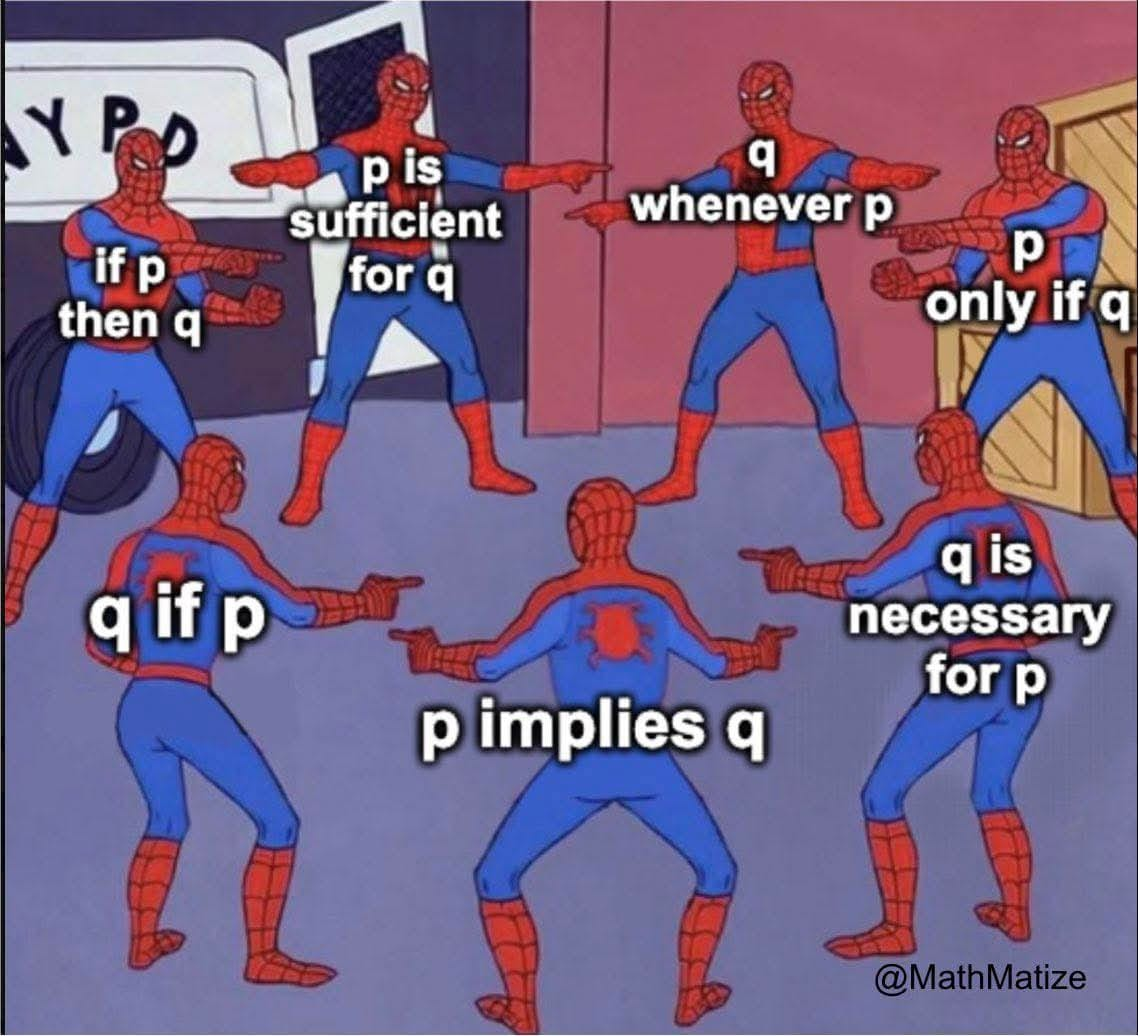
\includegraphics[width=0.8\linewidth,height=\textheight,keepaspectratio]{fig/fig10.jpg}
\caption{Source: Facebook}
\end{figure}

\subsubsection{\texorpdfstring{Truth Table for \(p \implies q\)}{Truth Table for p \textbackslash implies q}}\label{truth-table-for-p-implies-q}

\begin{longtable}[]{@{}
  >{\centering\arraybackslash}p{(\linewidth - 4\tabcolsep) * \real{0.2174}}
  >{\centering\arraybackslash}p{(\linewidth - 4\tabcolsep) * \real{0.2174}}
  >{\centering\arraybackslash}p{(\linewidth - 4\tabcolsep) * \real{0.5652}}@{}}
\toprule\noalign{}
\begin{minipage}[b]{\linewidth}\centering
\(p\)
\end{minipage} & \begin{minipage}[b]{\linewidth}\centering
\(q\)
\end{minipage} & \begin{minipage}[b]{\linewidth}\centering
\(p \implies q\)
\end{minipage} \\
\midrule\noalign{}
\endhead
\bottomrule\noalign{}
\endlastfoot
T & T & T \\
T & F & \textbf{F} \\
{F} & {T} & {T} \\
F & F & T \\
\end{longtable}

\begin{remark}
\leavevmode

\begin{itemize}
\tightlist
\item
  \(p \rightarrow q\) is \textbf{{ false} only when} \(p\) is true and \(q\) is false.
\item
  \(p \rightarrow q\) can be \textbf{true even if} \(p\) is false.
\item
  The truth of \(p \rightarrow q\) does \textbf{not require} that either \(p\) or \(q\) is true.
\end{itemize}

\end{remark}

\begin{example}
\protect\hypertarget{exm:unnamed-chunk-24}{}\label{exm:unnamed-chunk-24}

Consider the statement:\\
\textbf{``Employee pays taxes only if his income is more than 3 million.''}

Let:

\begin{itemize}
\tightlist
\item
  \(p\): Employee pays taxes\\
\item
  \(q\): His income is more than 3 million
\end{itemize}

Symbolically:

\[
p \implies q
\]

In other words:

\begin{itemize}
\tightlist
\item
  If employee pays taxes, then his income is more than 3 million.
\item
  Employee's income is more than 3 million, if he pays taxes.
\end{itemize}

\end{example}

\begin{example}
\protect\hypertarget{exm:unnamed-chunk-25}{}\label{exm:unnamed-chunk-25}Consider the statement:\\
\emph{``If \(n^2\) is even, then \(n\) is even.''}

Let:

\begin{itemize}
\tightlist
\item
  \(p\): \(n^2\) is even\\
\item
  \(q\): \(n\) is even
\end{itemize}

Symbolically:

\[
p \implies q
\]
\end{example}

\subsection{\texorpdfstring{Biconditional Logic: \(p \iff q\)}{Biconditional Logic: p \textbackslash iff q}}\label{biconditional-logic-p-iff-q}

\begin{definition}
\protect\hypertarget{def:unnamed-chunk-26}{}\label{def:unnamed-chunk-26}

Let \(p\) and \(q\) be propositions. The biconditional \(p \iff q\) is:

\begin{itemize}
\tightlist
\item
  \textbf{True} when \(p\) and \(q\) have the same truth value\\
\item
  \textbf{False} otherwise
\end{itemize}

\end{definition}

\begin{remark}

The statement \(p \iff q\) is true precisely when both \(p \Rightarrow q\) and \(q \Rightarrow p\) are true.\\
This is why we say:

\begin{itemize}
\tightlist
\item
  ``\(p\) if and only if \(q\)''\\
\item
  \(p \iff q \equiv (p \Rightarrow q) \land (q \Rightarrow p)\)
\end{itemize}

\end{remark}

\subsubsection{Alternate phrasing}\label{alternate-phrasing}

Not surprisingly, there are many ways of saying \(P \iff Q\) in English. The
following constructions all mean \(P \iff Q\):

\begin{itemize}
\tightlist
\item
  \(P\) if and only if \(Q\).
\item
  \(P\) is necessary and sufficient for \(Q\).
\item
  For \(P\) it is necessary and suffcient that \(Q\).
\item
  \(P\) is equivalent to \(Q\).
\item
  If \(P\), then \(Q\), and conversely.
\end{itemize}

The first three of these just combine constructions from the previous section
to express that\(P \implies Q\) and \(Q\implies  P\). In the last one, the words ``\emph{\ldots and conversely}'' mean that in addition to ``\emph{If \(P\), then \(Q\)}'' being true, the converse statement ``*If \(Q\), then \(P\)'' is also true.

\subsubsection{\texorpdfstring{Truth Table for \(p \iff q\)}{Truth Table for p \textbackslash iff q}}\label{truth-table-for-p-iff-q}

\begin{longtable}[]{@{}ccc@{}}
\toprule\noalign{}
\(p\) & \(q\) & \(p \iff q\) \\
\midrule\noalign{}
\endhead
\bottomrule\noalign{}
\endlastfoot
T & T & T \\
T & F & F \\
F & T & F \\
F & F & T \\
\end{longtable}

\begin{longtable}[]{@{}
  >{\centering\arraybackslash}p{(\linewidth - 8\tabcolsep) * \real{0.0826}}
  >{\centering\arraybackslash}p{(\linewidth - 8\tabcolsep) * \real{0.0826}}
  >{\centering\arraybackslash}p{(\linewidth - 8\tabcolsep) * \real{0.2149}}
  >{\centering\arraybackslash}p{(\linewidth - 8\tabcolsep) * \real{0.2149}}
  >{\centering\arraybackslash}p{(\linewidth - 8\tabcolsep) * \real{0.4050}}@{}}
\toprule\noalign{}
\begin{minipage}[b]{\linewidth}\centering
\(p\)
\end{minipage} & \begin{minipage}[b]{\linewidth}\centering
\(q\)
\end{minipage} & \begin{minipage}[b]{\linewidth}\centering
\(p \Rightarrow q\)
\end{minipage} & \begin{minipage}[b]{\linewidth}\centering
\(q \Rightarrow p\)
\end{minipage} & \begin{minipage}[b]{\linewidth}\centering
\((p \Rightarrow q) \land (q \Rightarrow p)\)
\end{minipage} \\
\midrule\noalign{}
\endhead
\bottomrule\noalign{}
\endlastfoot
T & T & T & T & T \\
T & F & F & T & F \\
F & T & T & F & F \\
F & F & T & T & T \\
\end{longtable}

\begin{example}
\protect\hypertarget{exm:unnamed-chunk-28}{}\label{exm:unnamed-chunk-28}\leavevmode

\begin{enumerate}
\def\labelenumi{\arabic{enumi}.}
\tightlist
\item
  ``A number is divisible by 2 if and only if it is even.''
\item
  ``A number being even is a necessary and sufficient condition for it to be divisible by 2.''
\end{enumerate}

\end{example}

\subsection{Terminology}\label{terminology}

Let the compound statement be:

**``If** \(p\), \textbf{then} \(q\)'' --- symbolically written as \(p \rightarrow q\)

Components

\begin{itemize}
\tightlist
\item
  \(p\): \textbf{Premise}, \textbf{Hypothesis}, or \textbf{Antecedent}
\item
  \(q\): \textbf{Conclusion} or \textbf{Consequent}
\end{itemize}

\begin{center}\rule{0.5\linewidth}{0.5pt}\end{center}

\begin{longtable}[]{@{}
  >{\raggedright\arraybackslash}p{(\linewidth - 4\tabcolsep) * \real{0.1680}}
  >{\raggedright\arraybackslash}p{(\linewidth - 4\tabcolsep) * \real{0.2080}}
  >{\raggedright\arraybackslash}p{(\linewidth - 4\tabcolsep) * \real{0.6240}}@{}}
\toprule\noalign{}
\begin{minipage}[b]{\linewidth}\raggedright
Transformation
\end{minipage} & \begin{minipage}[b]{\linewidth}\raggedright
Symbolic Form
\end{minipage} & \begin{minipage}[b]{\linewidth}\raggedright
Verbal Form
\end{minipage} \\
\midrule\noalign{}
\endhead
\bottomrule\noalign{}
\endlastfoot
\textbf{Converse} & \(q \rightarrow p\) & If \(q\), then \(p\) \\
\textbf{Inverse} & \(\neg p \rightarrow \neg q\) & If not \(p\), then not \(q\) \\
\textbf{Contrapositive} & \(\neg q \rightarrow \neg p\) & If not \(q\), then not \(p\) \\
\textbf{Negation} & \(p \land \neg q\) & \(p\) is true and \(q\) is false (i.e., the conditional fails) \\
\end{longtable}

\section{Truth Tables for Compound Propositions}\label{truth-tables-for-compound-propositions}

To analyze compound propositions:

\begin{itemize}
\tightlist
\item
  Use separate columns for each sub-expression.
\item
  Evaluate truth values for all combinations of truth values of the atomic propositions.
\item
  The final column shows the truth value of the entire compound proposition.
\end{itemize}

\begin{example}
\protect\hypertarget{exm:unnamed-chunk-29}{}\label{exm:unnamed-chunk-29}\leavevmode

\begin{quote}
\textbf{If a polygon is a triangle, then the sum of its angle measures is 180°}
\end{quote}

Let:

\begin{itemize}
\tightlist
\item
  \(p\): A polygon is a triangle\\
\item
  \(q\): The sum of the angle measures of a polygon is \(180^\circ\)
\end{itemize}

Then the compound statement is:

\begin{itemize}
\tightlist
\item
  \(p \implies q\)
\end{itemize}

\begin{enumerate}
\def\labelenumi{(\roman{enumi})}
\setcounter{enumi}{1}
\tightlist
\item
  \textbf{Converse}
\end{enumerate}

\begin{quote}
The converse of a conditional statement \(p \implies q\) is \(q \implies p\)
\end{quote}

\textbf{Statement}:\\
\textbf{If} the sum of the angle measures of a polygon is \(180^\circ\), \textbf{then} the polygon is a triangle.\\
\textbf{Symbolically}: \(q \implies p\)

\begin{enumerate}
\def\labelenumi{(\roman{enumi})}
\setcounter{enumi}{2}
\tightlist
\item
  \textbf{Inverse}
\end{enumerate}

\begin{quote}
The inverse of a conditional statement \(p \implies q\) is \(\neg p \implies \neg q\)
\end{quote}

\textbf{Statement}:\\
\textbf{If} a polygon is \textbf{not} a triangle, \textbf{then} the sum of its angle measures is \textbf{not} \(180^\circ\).\\
\textbf{Symbolically}:\\
\(\neg p \rightarrow \neg q\)

\begin{enumerate}
\def\labelenumi{(\roman{enumi})}
\setcounter{enumi}{3}
\tightlist
\item
  \textbf{Contrapositive}
\end{enumerate}

\begin{quote}
The contrapositive of a conditional statement \(p \implies q\) is \(\neg q \implies \neg p\)
\end{quote}

\textbf{Statement}:\\
\textbf{If} the sum of the angle measures of a polygon is \textbf{not} \(180^\circ\), \textbf{then} the polygon is \textbf{not} a triangle.\\
\textbf{Symbolically}: \(\neg q \implies \neg p\)

\begin{enumerate}
\def\labelenumi{(\alph{enumi})}
\setcounter{enumi}{21}
\tightlist
\item
  \textbf{Negation}
\end{enumerate}

\begin{quote}
The negation of a conditional statement \(p \implies q\) is \(p \land \neg q\)
\end{quote}

\textbf{Statement}:\\
A polygon \textbf{is} a triangle \textbf{and} the sum of its angle measures is \textbf{not} \(180^\circ\).\\
\textbf{Symbolically}: \(p \land \neg q\)

\end{example}

\section{Precedence of Logical Operations}\label{precedence-of-logical-operations}

To reduce parentheses in logical expressions, follow this precedence order:

\begin{longtable}[]{@{}ccc@{}}
\toprule\noalign{}
Operation & Symbol & Precedence \\
\midrule\noalign{}
\endhead
\bottomrule\noalign{}
\endlastfoot
Negation & \(\neg\) & 1 \\
Conjunction & \(\land\) & 2 \\
Disjunction & \(\lor\) & 3 \\
Implication & \(\Rightarrow\) & 4 \\
Biconditional & \(\Leftrightarrow\) & 5 \\
\end{longtable}

\begin{example}
\protect\hypertarget{exm:unnamed-chunk-30}{}\label{exm:unnamed-chunk-30}\leavevmode

\begin{itemize}
\item
  \(p \lor q \land r\) means:\(p \lor (q \land r)\)
\item
  \((p \lor q) \land r\) requires parentheses to override precedence.
\item
  \(p \lor q \Rightarrow \neg r\) means: \((p \lor q) \Rightarrow (\neg r)\)
\item
  \(p \lor (q \Rightarrow \neg r)\) requires parentheses to clarify grouping.
\end{itemize}

\end{example}

\begin{example}
\protect\hypertarget{exm:unnamed-chunk-31}{}\label{exm:unnamed-chunk-31}

Parse the statement\\
\((\neg p) \Rightarrow (p \lor (q \land p))\)

This uses:

\begin{itemize}
\tightlist
\item
  Negation on \(p\)
\item
  Conjunction \(q \land p\)
\item
  Disjunction \(p \lor (q \land p)\)
\item
  Implication from \(\neg p\) to the disjunction
\end{itemize}

\end{example}

\section{Truth Tables and Logical Analysis}\label{truth-tables-and-logical-analysis}

\subsection{Constructing a Truth Table}\label{constructing-a-truth-table}

To analyze a compound proposition:

\begin{enumerate}
\def\labelenumi{\arabic{enumi}.}
\item
  \textbf{Determine the number of atomic propositions}:\\
  If there are \(n\) propositions, the truth table will have \(2^n\) rows.
\item
  \textbf{List all combinations of truth values}:\\
  Fill the first \(n\) columns with all possible combinations of truth values for each proposition.
\item
  \textbf{Evaluate each sub-expression}:\\
  Add columns for intermediate steps and compute their truth values row by row.
\end{enumerate}

\begin{example}
\protect\hypertarget{exm:unnamed-chunk-32}{}\label{exm:unnamed-chunk-32}

Construct a truth table for the compound proposition:\\
\[
(p \lor \neg q) \Rightarrow (p \land q)
\]

\begin{longtable}[]{@{}
  >{\centering\arraybackslash}p{(\linewidth - 10\tabcolsep) * \real{0.0775}}
  >{\centering\arraybackslash}p{(\linewidth - 10\tabcolsep) * \real{0.0775}}
  >{\centering\arraybackslash}p{(\linewidth - 10\tabcolsep) * \real{0.1240}}
  >{\centering\arraybackslash}p{(\linewidth - 10\tabcolsep) * \real{0.1860}}
  >{\centering\arraybackslash}p{(\linewidth - 10\tabcolsep) * \real{0.1550}}
  >{\centering\arraybackslash}p{(\linewidth - 10\tabcolsep) * \real{0.3798}}@{}}
\toprule\noalign{}
\begin{minipage}[b]{\linewidth}\centering
\(p\)
\end{minipage} & \begin{minipage}[b]{\linewidth}\centering
\(q\)
\end{minipage} & \begin{minipage}[b]{\linewidth}\centering
\(\neg q\)
\end{minipage} & \begin{minipage}[b]{\linewidth}\centering
\(p \lor \neg q\)
\end{minipage} & \begin{minipage}[b]{\linewidth}\centering
\(p \land q\)
\end{minipage} & \begin{minipage}[b]{\linewidth}\centering
\((p \lor \neg q) \Rightarrow (p \land q)\)
\end{minipage} \\
\midrule\noalign{}
\endhead
\bottomrule\noalign{}
\endlastfoot
T & T & F & T & T & T \\
T & F & T & T & F & F \\
F & T & F & F & F & T \\
F & F & T & T & F & F \\
\end{longtable}

\end{example}

\begin{remark}
To construct the truth table for a given proposition:
1 . Create a table with \(2^n\) rows if a compound proposition involves \(n\).
propsitions.
2. Fill in the first \(n\) columns with all possible cobinations.
3. Determine and enter the truth value for each combination.
\end{remark}

\begin{example}
\protect\hypertarget{exm:unnamed-chunk-34}{}\label{exm:unnamed-chunk-34}For \(n=3\),

This table lists all possible combinations of truth values for three atomic propositions: \(p\), \(q\), and \(r\).

\[
\begin{array}{|c|c|c|}
\hline
p & q & r \\
\hline
T & T & T \\
F & T & T \\
T & F & T \\
F & F & T \\
T & T & F \\
F & T & F \\
T & F & F \\
F & F & F \\
\hline
\end{array}
\]
\end{example}

\begin{exercise}
\protect\hypertarget{exr:unnamed-chunk-35}{}\label{exr:unnamed-chunk-35}

Construct truth tables for the following compound propositions

\begin{enumerate}
\def\labelenumi{\alph{enumi})}
\item
  \[
  \neg (P \lor Q) \lor (\neg P)
  \]
\item
  \[
  \neg (P \Rightarrow Q)
  \]
\item
  \[
  P \lor (Q \Rightarrow R)
  \]
\end{enumerate}

\end{exercise}

\begin{exercise}
\protect\hypertarget{exr:unnamed-chunk-36}{}\label{exr:unnamed-chunk-36}Suppose the statement \(((P \land Q) \lor R) \Rightarrow (R \lor S)\) is \textbf{false}.\\
Find the truth values of \(P\), \(Q\), \(R\), and \(S\) without constructing a full truth table.
\end{exercise}

\section{Tautologies and Contradictions}\label{tautologies-and-contradictions}

\begin{definition}
\protect\hypertarget{def:unnamed-chunk-37}{}\label{def:unnamed-chunk-37}\leavevmode

\begin{itemize}
\tightlist
\item
  A \textbf{tautology} is a compound proposition that is always true, regardless of the truth values of its components.
\item
  A \textbf{contradiction} is a compound proposition that is always false.
\item
  A \textbf{contingency} is a compound proposition that is neither a tautology nor a contradiction.
\end{itemize}

\end{definition}

\begin{example}
\protect\hypertarget{exm:unnamed-chunk-38}{}\label{exm:unnamed-chunk-38}Let \(p\): ``This course is easy.''

\begin{enumerate}
\def\labelenumi{(\roman{enumi})}
\tightlist
\item
  Contradiction:\\
  ``This course is easy \textbf{and} this course is not easy''\\
  Expression: \(p \land \neg p\)
\end{enumerate}

\[
\begin{array}{|c|c|c|}
\hline
p & \neg p & p \land \neg p \\
\hline
T & F & F \\
F & T & F \\
\hline
\end{array}
\]

\begin{enumerate}
\def\labelenumi{(\roman{enumi})}
\setcounter{enumi}{1}
\tightlist
\item
  Tautology:\\
  ``This course is easy \textbf{or} this course is not easy''\\
  Expression: \(p \lor \neg p\)
\end{enumerate}

\[
\begin{array}{|c|c|}
\hline
p & p \lor \neg p \\
\hline
T & T \\
F & T \\
\hline
\end{array}
\]
\end{example}

\section{Logical Equivalence}\label{logical-equivalence}

\begin{definition}
\protect\hypertarget{def:unnamed-chunk-39}{}\label{def:unnamed-chunk-39}Two compound propositions \(p\) and \(q\) are \textbf{logically equivalent} if they yield the same truth values for all combinations of truth values of their components. Denoted as:

\[
p \equiv q
\]
\end{definition}

\begin{remark}
\leavevmode

\begin{itemize}
\tightlist
\item
  \(p \equiv q\) means that \(p \iff q\) is a tautology.
\item
  The symbol \(\equiv\) is not a logical connective; it asserts that the biconditional \(p \iff q\) is always true.
\end{itemize}

\end{remark}

\subsection{Useful Logical Equivalences}\label{useful-logical-equivalences}

These equivalences are foundational in propositional logic and are often used to simplify or transform logical expressions.

\begin{enumerate}
\def\labelenumi{\arabic{enumi}.}
\item
  \textbf{Double Negation}\\
  \[
  \neg(\neg p) \equiv p
  \]
\item
  \textbf{De Morgan's Law (Conjunction)}\\
  \[
  \neg(p \land q) \equiv \neg p \lor \neg q
  \]
\item
  \textbf{De Morgan's Law (Disjunction)}\\
  \[
  \neg(p \lor q) \equiv \neg p \land \neg q
  \]
\item
  \textbf{Implication}\\
  \[
  p \Rightarrow q \equiv \neg p \lor q
  \]
\item
  \textbf{Negation of Implication}\\
  \[
  \neg(p \Rightarrow q) \equiv p \land \neg q
  \]
\end{enumerate}

\section{The Algebra of Propositions}\label{the-algebra-of-propositions}

\section{The Algebra of Propositions}\label{the-algebra-of-propositions-1}

\subsection{Logical Laws and Their Equivalences}\label{logical-laws-and-their-equivalences}

\begin{longtable}[]{@{}
  >{\raggedright\arraybackslash}p{(\linewidth - 4\tabcolsep) * \real{0.1608}}
  >{\raggedright\arraybackslash}p{(\linewidth - 4\tabcolsep) * \real{0.4196}}
  >{\raggedright\arraybackslash}p{(\linewidth - 4\tabcolsep) * \real{0.4196}}@{}}
\toprule\noalign{}
\begin{minipage}[b]{\linewidth}\raggedright
Law Name
\end{minipage} & \begin{minipage}[b]{\linewidth}\raggedright
Disjunction-related Expression(s)
\end{minipage} & \begin{minipage}[b]{\linewidth}\raggedright
Conjunction-related Expression(s)
\end{minipage} \\
\midrule\noalign{}
\endhead
\bottomrule\noalign{}
\endlastfoot
\textbf{Idempotent Laws} & \(p \lor p \equiv p\) & \(p \land p \equiv p\) \\
\textbf{Associative Laws} & \((p \lor q) \lor r \equiv p \lor (q \lor r)\) & \((p \land q) \land r \equiv p \land (q \land r)\) \\
\textbf{Commutative Laws} & \(p \lor q \equiv q \lor p\) & \(p \land q \equiv q \land p\) \\
\textbf{Distributive Laws} & \(p \lor (q \land r) \equiv (p \lor q) \land (p \lor r)\) & \(p \land (q \lor r) \equiv (p \land q) \lor (p \land r)\) \\
\textbf{Identity Laws} & \(p \lor F \equiv p\), \(p \lor T \equiv T\) & \(p \land F \equiv F\), \(p \land T \equiv p\) \\
\textbf{Involution Law} & --- & \(\neg \neg p \equiv p\) \\
\textbf{Complement Laws} & \(\neg p \lor p \equiv T\) & \(\neg p \land p \equiv F\) \\
\textbf{De Morgan's Laws} & \(\neg (p \land q) \equiv \neg p \lor \neg q\) & \(\neg (p \lor q) \equiv \neg p \land \neg q\) \\
\textbf{Conditional Identities} & \(p \Rightarrow q \equiv \neg p \lor q\) & \(p \Leftrightarrow q \equiv (p \Rightarrow q) \land (q \Rightarrow p)\) \\
\end{longtable}

\begin{example}
\protect\hypertarget{exm:unnamed-chunk-41}{}\label{exm:unnamed-chunk-41}\leavevmode

\begin{enumerate}
\def\labelenumi{\arabic{enumi}.}
\item
  Show that:\\
  \[
  p \land \neg (q \Rightarrow \neg r) \equiv p \land (q \land r)
  \]
\item
  Show that:\\
  \[
  p \Leftrightarrow q \equiv \neg q \Leftrightarrow \neg p
  \]
\item
  Using logically equivalent statements (without truth tables), show:\\
  \[
  \neg (\neg p \land q) \land (p \lor q) \equiv p
  \]
\end{enumerate}

\end{example}

\section{Predicate Logic and Quantifiers}\label{predicate-logic-and-quantifiers}

Consider the following statements:

\[
x > 3, \quad x = y + 3, \quad x + y = z
\]

The truth value of these statements has no meaning without specifying the values of \(x, y, z\).

However, we can make propositions out of such statements.

A \textbf{predicate} is a property that is true or false about the subject (in logic, we say ``variable'') of a statement.

For example:

\[
\text{``} \quad \underbrace{x}_{\text{subject}} \quad \underbrace{\text{is greater than 3"}}_{\text{predicate}} 
\]

\subsection{Predicates}\label{predicates}

A \textbf{predicate} is a declarative sentence whose truth value depends on one or more variables.

The statement:
\[
x \text{ is greater than } 3
\]

has two parts:

\begin{itemize}
\tightlist
\item
  The \textbf{predicate}: ``is greater than 3''
\item
  The \textbf{variable}: \(x\)
\end{itemize}

We denote this statement by \(P(x)\), where:

\begin{itemize}
\tightlist
\item
  \(P\) is the predicate ``is greater than 3''
\item
  \(x\) is the variable
\end{itemize}

By assigning a value to \(x\), \(P(x)\) becomes a \textbf{proposition} with a definite truth value:

\begin{itemize}
\tightlist
\item
  \(P(5)\): ``5 is greater than 3'' → \textbf{True}
\item
  \(P(2)\): ``2 is greater than 3'' → \textbf{False}
\end{itemize}

\textbf{Note}:

\begin{itemize}
\tightlist
\item
  A \textbf{predicate} is neither true nor false on its own.
\item
  A predicate becomes a \textbf{proposition} when its variables are substituted with specific values.
\item
  The \textbf{domain} (also called the universe or universe of discourse) of a predicate variable is the set of all values that may be substituted for the variable.
\end{itemize}

\begin{definition}
\protect\hypertarget{def:unnamed-chunk-42}{}\label{def:unnamed-chunk-42}Let \(A\) be a nonempty set. An expression \(P(x)\) defined on \(A\) is called a \textbf{predicate} if:

\[
P(a) \text{ is either true or false for each } a \in A
\]

That is, \(P(a)\) becomes a \textbf{statement} (i.e., a proposition with a definite truth value) whenever any element \(a \in A\) is substituted for the variable \(x\).
\end{definition}

\begin{example}
\protect\hypertarget{exm:unnamed-chunk-43}{}\label{exm:unnamed-chunk-43}

\textbf{(i)} Let \(P(x): x^2 > 6\), where \(x \in \mathbb{N}\)

\begin{itemize}
\tightlist
\item
  \(P(1)\): \(1^2 = 1 \not> 6\) → False\\
\item
  \(P(2)\): \(2^2 = 4 \not> 6\) → False\\
\item
  For \(x \in \mathbb{N}\) and \(x \ne 1, x \ne 2\), \(P(x)\) is true.
\end{itemize}

\textbf{(ii)} Let \(P(x, y): x^2 + y^2 = 4\), where \(x, y \in \mathbb{R}\)

\begin{itemize}
\tightlist
\item
  \(P(0, 2)\): \(0^2 + 2^2 = 4\) → True\\
\item
  \(P(1, 1)\): \(1^2 + 1^2 = 2\) → False
\end{itemize}

\end{example}

\subsection{Converting Predicates to Propositions}\label{converting-predicates-to-propositions}

There are two standard methods:

\begin{enumerate}
\def\labelenumi{\arabic{enumi}.}
\item
  \textbf{Assign specific values to variables}\\
  Example: \(P(3)\), \(P(0, 2)\)
\item
  \textbf{Add quantifiers}

  \begin{itemize}
  \tightlist
  \item
    Universal: \(\forall x \in \mathbb{N},\; P(x)\)\\
  \item
    Existential: \(\exists x \in \mathbb{R},\; P(x)\)
  \end{itemize}
\end{enumerate}

\pandocbounded{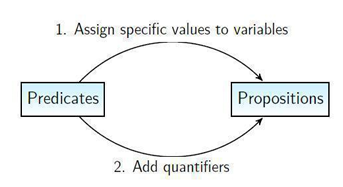
\includegraphics[keepaspectratio]{fig/fig1.png}}

\section{Quantifiers}\label{quantifiers}

A predicate becomes a proposition when we assign it fixed values. However, another way to convert a predicate into a proposition is by \textbf{quantifying} it.

Quantification expresses whether a predicate is true for:

\begin{itemize}
\tightlist
\item
  \textbf{All} values in the universe of discourse
\item
  \textbf{Some} values in the universe of discourse
\end{itemize}

\begin{definition}
\protect\hypertarget{def:unnamed-chunk-44}{}\label{def:unnamed-chunk-44}\textbf{Quantifiers} are words that refer to quantities such as ``all'' or ``some.'' They indicate how many elements in the domain satisfy a given predicate.
\end{definition}

Two Types of Quantifiers

\begin{enumerate}
\def\labelenumi{\arabic{enumi}.}
\tightlist
\item
  \textbf{Universal Quantifier}\\
  Symbol: \(\forall\)\\
  Meaning: ``For all'' or ``For every,'' or ``For each,''
  Example:
\end{enumerate}

\begin{quote}
For every \(n \in \mathbb{Z}\), \(2n\) is even.
\end{quote}

This can be expressed symbolically as:

\[
\forall n \in \mathbb{Z},\; 2n \text{ is even}
\]

\begin{enumerate}
\def\labelenumi{\arabic{enumi}.}
\setcounter{enumi}{1}
\tightlist
\item
  \textbf{Existential Quantifier}\\
  Symbol: \(\exists\)\\
  Meaning: ``There exists a'' or ``There is a.''\\
  Example:
\end{enumerate}

\begin{quote}
There exists an integer \(n \in \mathbb{Z}\) such that \(n^2 = 2\).
\end{quote}

This can be expressed symbolically as:

\[
\exists n \in \mathbb{Z},\; n^2 = 2
\]

\subsection{\texorpdfstring{Universal Quantifier \(\forall\)}{Universal Quantifier \textbackslash forall}}\label{universal-quantifier-forall}

Let \(p(x)\) be a predicate, where \(x \in D\).

Suppose the statement\\
\textgreater{} ``For any \(x\) in a non-empty subset \(S \subseteq D\), \(p(x)\) is true''\\
is valid.

Then the expression\\
\[
\forall x \in S,\; p(x)
\]\\
is a \textbf{proposition}.

This means:\\
\textgreater{} ``For every \(x\) in the subset \(S\), the predicate \(p(x)\) holds.''

\begin{example}
\protect\hypertarget{exm:unnamed-chunk-45}{}\label{exm:unnamed-chunk-45}Let \(p(x)\): ``\(x\) is even''\\
Let \(D = \{1, 2, 3, 4, 5, 6, 7, 8, 9, 10\}\)\\
Let \(S = \{2, 4, 6, 8, 10\} \subseteq D\)

Then:
\[
\forall x \in S,\; p(x)
\]
is true, since all elements of \(S\) are even.
\end{example}

\subsubsection{Notation}\label{notation}

\begin{itemize}
\tightlist
\item
  \(\forall x\; P(x)\): Read as ``for all \(x\), \(P(x)\)'' or ``for every \(x\), \(P(x)\)''
\item
  \(\forall\): Universal quantifier
\end{itemize}

\begin{definition}
\protect\hypertarget{def:unnamed-chunk-46}{}\label{def:unnamed-chunk-46}An element \(x\) for which \(P(x)\) is false is called a counterexample of \(\forall x P(x)\).
\end{definition}

\subsubsection{\texorpdfstring{Other ways to say \(\forall\)}{Other ways to say \textbackslash forall}}\label{other-ways-to-say-forall}

\begin{itemize}
\tightlist
\item
  All of\ldots{}
\item
  For each\ldots{}
\item
  Given any\ldots{}
\item
  For any\ldots{}
\item
  For arbitrary\ldots{}
\end{itemize}

\begin{example}
\protect\hypertarget{exm:unnamed-chunk-47}{}\label{exm:unnamed-chunk-47}Let \(P(x): x^2 > x\), where \(x\) is a real number.

Then ``\(\forall x\, P(x)\)'' in English means ``for all \(x\), \(x^2 > x\)'', or we can say ``for any \(x\), \(x^2 > x\)'', or in other words ``given any \(x\), \(x^2 > x\)''.

An element \(x = \frac{1}{2}\), since \(\left(\frac{1}{2}\right)^2 = \frac{1}{4} < \frac{1}{2}\), is false. That is, \(P\left(\frac{1}{2}\right)\) is false.

So, \(x = \frac{1}{2}\) is a counterexample to the statement ``for all \(x\), \(x^2 > x\)'', where \(x\) is a real number.
\end{example}

\begin{example}
\protect\hypertarget{exm:unnamed-chunk-48}{}\label{exm:unnamed-chunk-48}Consider the predicate \(|x| \geq 0\), where \(x \in \mathbb{R}\).

Let \(P(x): |x| \geq 0\).

Then, \(\forall x \in \mathbb{R},\, P(x)\) is true.

i.e., \(\forall x \in \mathbb{R},\, |x| \geq 0\).
\end{example}

\begin{example}
\protect\hypertarget{exm:unnamed-chunk-49}{}\label{exm:unnamed-chunk-49}Consider the predicate \(x > \frac{1}{2}\), where \(x \in \mathbb{R}\).

Let \(P(x): x > \frac{1}{2}\).

Then \(\forall x \in \mathbb{R},\, P(x)\) is false, since for instance \(0 \in \mathbb{R}\), but \(P(0)\) is false.

i.e., \(\neg (\forall x \in \mathbb{R},\, P(x))\).

However, \(\forall x \in \mathbb{N},\, P(x)\) is true.

i.e., \(\forall x \in \mathbb{N},\, P(x)\).
\end{example}

\subsection{\texorpdfstring{The Existential Quantifier ``\(\exists\)''}{The Existential Quantifier ``\textbackslash exists''}}\label{the-existential-quantifier-exists}

Let \(p(x)\) be a predicate, where \(x \in D\).

Suppose:\\
``There is \(x_0 \in S \subseteq D\), such that \(p(x_0)\)'' is true.

Then:\\
``There is \(x_0 \in S \subseteq D\), such that \(p(x_0)\)'' is a proposition.

We write this proposition as:

\[ \exists x_0 \in S,\ p(x_0) \]

Which means:\\
``There exists \(x_0 \in S\) such that \(p(x_0)\)'' is true.

i.e.,

\[ \exists x_0 \in S,\ p(x_0) \]

\subsubsection{Notation}\label{notation-1}

\(\exists x\, P(x)\), where \(\exists\) is called the existential quantifier.

\subsubsection{\texorpdfstring{Other ways to read \(\exists\):}{Other ways to read \textbackslash exists:}}\label{other-ways-to-read-exists}

\begin{itemize}
\tightlist
\item
  ``There is an \(x\) such that \(P(x)\).''
\item
  ``There is at least one \(x\) such that \(P(x)\).''
\item
  ``For some \(x\), \(P(x)\).''
\end{itemize}

\begin{example}
\protect\hypertarget{exm:unnamed-chunk-50}{}\label{exm:unnamed-chunk-50}Consider the predicate \(2x > 7\), where \(x \in \mathbb{N}\).

Let \(P(x): 2x > 7\).

When \(x \in \mathbb{N}\) and \(2x > 7\) is true (since \(10 > 7\)),

i.e., when \(x = 5\), \(x \in \mathbb{N}\) and \(P(5)\) is true.

Therefore,

\[ \exists x \in \mathbb{N},\ P(x) \text{ is true} \]

i.e.,

\[ \exists x \in \mathbb{N},\ 2x > 7 \]
\end{example}

\begin{example}
\protect\hypertarget{exm:unnamed-chunk-51}{}\label{exm:unnamed-chunk-51}Consider the predicate \(x^2 > 1\), where \(x \in \mathbb{R}\).

Let \(A = \{0, 1, -1\}\) and define \(P(x): x^2 > 1\).

Then:
- \(P(0)\) is false,
- \(P(1)\) is false,
- \(P(-1)\) is false.

Therefore,

\[ \exists x \in A,\ P(x) \]

is false,

i.e.,

\[ \neg (\exists x \in A,\ P(x)) \]

.

However,

\[ \exists x \in \mathbb{N},\ P(x) \]

is true,\\
since when \(x = 2\), \(x \in \mathbb{N}\) and \(P(2)\) is true.

i.e.,

\[ \exists x \in \mathbb{N},\ x^2 > 1. \]
\end{example}

Let \(p(x)\) be a predicate and \(D\) be the domain of \(x\).

An existential statement is a statement of the form:

\[ \exists x \in D,\ p(x) \]

\begin{itemize}
\tightlist
\item
  Forms:

  \begin{itemize}
  \tightlist
  \item
    ``There exists an \(x\) such that \(p(x)\)''
  \item
    ``For some \(x\), \(p(x)\)''
  \item
    ``We can find an \(x\) such that \(p(x)\)''
  \item
    ``There is some \(x\) such that \(p(x)\)''
  \item
    ``There is at least one \(x\) such that \(p(x)\)''
  \end{itemize}
\item
  The statement is \textbf{true} if \(p(x)\) is true for \textbf{at least one} \(x \in D\).
\item
  The statement is \textbf{false} if \(p(x)\) is false for \textbf{all} \(x \in D\).
\item
  A \textbf{Counterproof} to disprove an existential statement, one must show that \(p(x)\) is false for \textbf{every} \(x \in D\).
\end{itemize}

\subsection{Quantifiers and Negation}\label{quantifiers-and-negation}

Suppose \(A\) is a non-empty set, \(P(x)\) is a predicate where \(x \in A\), and \(B \subseteq A\) is a non-empty subset.

We consider the negations of quantified statements:

\begin{enumerate}
\def\labelenumi{\arabic{enumi}.}
\tightlist
\item
  Negation of a Universal Statement
\end{enumerate}

\[
\neg (\forall x \in B,\ P(x))
\]

This means:\\
It is not the case that for every \(x \in B\), \(P(x)\) holds.\\
So, there exists some \(x \in B\) such that \(P(x)\) does not hold:

\[
\exists x \in B,\ \neg P(x)
\]

\begin{enumerate}
\def\labelenumi{\arabic{enumi}.}
\setcounter{enumi}{1}
\tightlist
\item
  Negation of an Existential Statement
\end{enumerate}

\[
\neg (\exists x \in B,\ P(x))
\]

This means:\\
It is not the case that there exists some \(x \in B\) such that \(P(x)\) holds.\\
So, for every \(x \in B\), \(P(x)\) does not hold:

\[
\forall x \in B,\ \neg P(x)
\]

The following equivalences hold:

\[ \neg (\forall x \in B,\ P(x)) \equiv \exists x \in B,\ \neg P(x) \]
\[ \neg (\exists x \in B,\ P(x)) \equiv \forall x \in B,\ \neg P(x) \]

\begin{itemize}
\item
  \(\neg (\forall x \in D,\ p(x)) \equiv \exists x \in D,\ \neg p(x)\)
\item
  \(\neg (\exists x \in D,\ p(x)) \equiv \forall x \in D,\ \neg p(x)\)
\item
  The negation of a universal statement (``all are'') is logically equivalent to an existential statement (``there is at least one that is not'').
\item
  The negation of an existential statement (``some are'') is logically equivalent to a universal statement (``all are not'').
\end{itemize}

\begin{example}
\protect\hypertarget{exm:unnamed-chunk-52}{}\label{exm:unnamed-chunk-52}\leavevmode

\begin{itemize}
\item
  \(\forall\) primes \(p\), \(p\) is odd\\
  \textbf{Negation:} \(\exists\) prime \(p\), \(p\) is even
\item
  \(\exists\) triangle \(T\), the sum of angles of \(T\) equals \(200^\circ\)\\
  \textbf{Negation:} \(\forall\) triangles \(T\), the sum of angles of \(T\) does not equal \(200^\circ\)
\end{itemize}

\end{example}

\subsubsection{Truth Value of Quantified Statements}\label{truth-value-of-quantified-statements}

\begin{longtable}[]{@{}
  >{\raggedright\arraybackslash}p{(\linewidth - 4\tabcolsep) * \real{0.1927}}
  >{\raggedright\arraybackslash}p{(\linewidth - 4\tabcolsep) * \real{0.3945}}
  >{\raggedright\arraybackslash}p{(\linewidth - 4\tabcolsep) * \real{0.4128}}@{}}
\toprule\noalign{}
\begin{minipage}[b]{\linewidth}\raggedright
Statement
\end{minipage} & \begin{minipage}[b]{\linewidth}\raggedright
When True
\end{minipage} & \begin{minipage}[b]{\linewidth}\raggedright
When False
\end{minipage} \\
\midrule\noalign{}
\endhead
\bottomrule\noalign{}
\endlastfoot
\(\forall x \in D,\ P(x)\) & \(P(x)\) is true for every \(x \in D\) & There exists at least one \(x \in D\) such that \(P(x)\) is false \\
\(\exists x \in D,\ P(x)\) & There exists at least one \(x \in D\) such that \(P(x)\) is true & \(P(x)\) is false for every \(x \in D\) \\
\end{longtable}

\begin{example}
\protect\hypertarget{exm:unnamed-chunk-53}{}\label{exm:unnamed-chunk-53}

We are given the logical equivalence:
\[
\neg (\exists x\ \forall y\ \exists z\ P(x, y, z)) \equiv \forall x\ \exists y\ \forall z\ \neg P(x, y, z)
\]

\pandocbounded{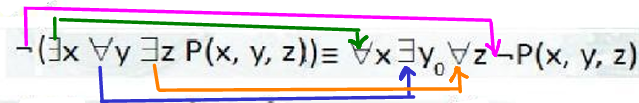
\includegraphics[keepaspectratio]{fig/fig2.png}}

\end{example}

\textbf{Note}:
Logical operations from propositional logic --- such as \(\neg\), \(\land\), \(\lor\), \(\Rightarrow\), \(\Leftrightarrow\) ---\\
can also be applied to quantified statements.

Here is a clean transcription of the image content, showing only the questions and definitions without any answers or reformulations:

\begin{center}\rule{0.5\linewidth}{0.5pt}\end{center}

\subsection{Negation of Quantification}\label{negation-of-quantification}

Given a quantified statement of the form:

\[
\neg(\forall x \in D,\, P(x) \land Q(x))
\]

Apply logical transformations to express its equivalent forms.

\subsubsection{Conditional Quantification}\label{conditional-quantification}

Consider the conditional quantification:

\[
\forall x \in D,\, P(x) \Rightarrow Q(x)
\]

Define the following related forms:

\begin{itemize}
\item
  \textbf{Converse}: \(\forall x \in D,\, Q(x) \Rightarrow P(x)\)
\item
  \textbf{Contrapositive}: \(\forall x \in D,\, \neg Q(x) \Rightarrow \neg P(x)\)
\item
  \textbf{Inverse}:\(\forall x \in D,\, \neg P(x) \Rightarrow \neg Q(x)\)
\end{itemize}

\textbf{Note}: : A conditional proposition is logically equivalnce to its contrapositive.

\[
\forall x \in D, P(x) \implies Q(x)\equiv \forall x\in D, \neg Q(x) \implies \neg P(x)
\]

\subsection{Negation of Conditional Quantification}\label{negation-of-conditional-quantification}

\begin{align}
\neg (\forall x \in D, P(x) \implies Q(x)) &\equiv \exists x_0 \in D \neg (P(x_0) \implies Q(x_0))\\
& \equiv \exists x_0 \in D P(x_0) \land  \neg Q(x_0)
\end{align}

\begin{example}
\protect\hypertarget{exm:unnamed-chunk-54}{}\label{exm:unnamed-chunk-54}

Let \(x \in \mathbb{R}\).

\begin{itemize}
\item
  \(x = 1\) is a sufficient condition for \(x^2 = 1\)\\
  i.e., \(\forall x \in \mathbb{R},\ x = 1 \Rightarrow x^2 = 1\)
\item
  \(x^2 = 1\) is a necessary condition for \(x = 1\)\\
  i.e., \(\forall x \in \mathbb{R},\ x^2 \neq 1 \Rightarrow x \neq 1\)
\item
  \(x = 1\) only if \(x^2 = 1\)\\
  i.e., \(\forall x \in \mathbb{R},\ x^2 \neq 1 \Rightarrow x \neq 1\)
\end{itemize}

\end{example}

\begin{example}
\protect\hypertarget{exm:unnamed-chunk-55}{}\label{exm:unnamed-chunk-55}Let \(x \in \mathbb{R}\).

Statement: \(\forall x,\ x > 10 \Rightarrow x^2 > 100\)

Negation: \(\exists x \in \mathbb{R}\) such that \(x > 10\) and \(x^2 \leq 100\)
\end{example}

\begin{example}
\protect\hypertarget{exm:unnamed-chunk-56}{}\label{exm:unnamed-chunk-56}Let \(x \in \mathbb{R}\).

Statement:\\
If \(x > 1\), then \(x^2 > 1\)

Define:\\
\(P(x): x > 1\)\\
\(Q(x): x^2 > 1\)

Symbolic form:

\[
\forall x \in \mathbb{R},\ P(x) \Rightarrow Q(x)
\]

Negation:

\[
\exists x_0 \in \mathbb{R},\ P(x_0) \land \neg Q(x_0)
\]

i.e.,

\[
x_0 > 1 \quad \text{and} \quad x_0^2 \leq 1
\]
\end{example}

\chapter{Introduction to Proofs}\label{introduction-to-proofs}

\subsection{Terminology}\label{terminology-1}

\begin{itemize}
\tightlist
\item
  \textbf{Theorem}: A statement that can be shown to be true (i.e., a fact or result).
\item
  \textbf{Proposition}: A smaller or less important theorem.
\item
  \textbf{Axiom / Postulate}: A statement assumed to be true.
\item
  \textbf{Lemma}: A less important theorem used in the proof of another theorem.
\item
  \textbf{Corollary}: A less important theorem that follows from a larger theorem.
\item
  \textbf{Conjecture}: A statement proposed as true but not yet proven.
\end{itemize}

\textbf{Note}: A \textbf{proof} is a valid argument that establishes the truth of a theorem (or any statement that can be true or false).\\
Axioms and postulates do not require proof---they serve as foundational assumptions, akin to basic words in a dictionary that help define others.

\section{Arguments}\label{arguments}

\begin{itemize}
\item
  An \textbf{argument} is an assertion that a given set of propositions \(p_1, p_2, \ldots, p_n\), called \textbf{premises}, yields another proposition \(q\), called the \textbf{conclusion}.
\item
  This is denoted symbolically as:
  \[
  p_1, p_2, \ldots, p_n \vdash q
  \]
\item
  The argument is said to be \textbf{valid} if \(q\) is true whenever all the premises \(p_1, p_2, \ldots, p_n\) are true.
\item
  An argument that is not valid is called a \textbf{fallacy}.
\item
  The argument \(p_1, p_2, \ldots, p_n \vdash q\) is \textbf{valid} if and only if the compound proposition:
  \[
  (p_1 \land p_2 \land \ldots \land p_n) \Rightarrow q
  \]
  is a \textbf{tautology}.
\end{itemize}

\begin{example}
\protect\hypertarget{exm:unnamed-chunk-57}{}\label{exm:unnamed-chunk-57}Let \(n \in \mathbb{N}\). Consider the following argument:

\begin{enumerate}
\def\labelenumi{\arabic{enumi}.}
\tightlist
\item
  \((-1)^n\) is positive or \((-1)^n\) is negative.\\
\item
  If \((-1)^n\) is positive, then \((-1)^{2n} > 0\).\\
\item
  If \((-1)^n\) is negative, then \((-1)^{2n} > 0\).
\end{enumerate}

Therefore, \((-1)^{2n} > 0\).

Let:
- \(p\): \((-1)^n\) is positive\\
- \(q\): \((-1)^n\) is negative\\
- \(r\): \((-1)^{2n} > 0\)

We examine the validity of the argument:
\[
\underbrace{(p \lor q)}_{Premise},\ \underbrace{(p \Rightarrow r)}_{Premise},\ \underbrace{(q \Rightarrow r)}_{Premise} \vdash \underbrace{r}_{Conclusion}
\]

This corresponds to the compound proposition:
\[
((p \lor q) \land (p \Rightarrow r) \land (q \Rightarrow r)) \Rightarrow r
\]

\begin{longtable}[]{@{}
  >{\centering\arraybackslash}p{(\linewidth - 14\tabcolsep) * \real{0.0343}}
  >{\centering\arraybackslash}p{(\linewidth - 14\tabcolsep) * \real{0.0343}}
  >{\centering\arraybackslash}p{(\linewidth - 14\tabcolsep) * \real{0.0343}}
  >{\centering\arraybackslash}p{(\linewidth - 14\tabcolsep) * \real{0.0687}}
  >{\centering\arraybackslash}p{(\linewidth - 14\tabcolsep) * \real{0.0987}}
  >{\centering\arraybackslash}p{(\linewidth - 14\tabcolsep) * \real{0.0987}}
  >{\centering\arraybackslash}p{(\linewidth - 14\tabcolsep) * \real{0.2790}}
  >{\centering\arraybackslash}p{(\linewidth - 14\tabcolsep) * \real{0.3519}}@{}}
\toprule\noalign{}
\begin{minipage}[b]{\linewidth}\centering
\(p\)
\end{minipage} & \begin{minipage}[b]{\linewidth}\centering
\(q\)
\end{minipage} & \begin{minipage}[b]{\linewidth}\centering
\(r\)
\end{minipage} & \begin{minipage}[b]{\linewidth}\centering
\(p \lor q\)
\end{minipage} & \begin{minipage}[b]{\linewidth}\centering
\(p \Rightarrow r\)
\end{minipage} & \begin{minipage}[b]{\linewidth}\centering
\(q \Rightarrow r\)
\end{minipage} & \begin{minipage}[b]{\linewidth}\centering
\((p \lor q) \land (p \Rightarrow r) \land (q \Rightarrow r)\)
\end{minipage} & \begin{minipage}[b]{\linewidth}\centering
\(((p \lor q) \land (p \Rightarrow r) \land (q \Rightarrow r)) \Rightarrow r\)
\end{minipage} \\
\midrule\noalign{}
\endhead
\bottomrule\noalign{}
\endlastfoot
T & T & T & T & T & T & T & T \\
F & T & T & T & T & T & T & T \\
T & F & T & T & T & T & T & T \\
F & F & T & F & T & T & F & T \\
T & T & F & T & F & F & F & F \\
T & F & F & T & F & T & F & F \\
F & T & F & T & T & F & F & F \\
F & F & F & F & T & T & F & T \\
\end{longtable}

This table confirms that the compound proposition is \textbf{not} a tautology, hence the argument is \textbf{not valid} in all cases. However, in the specific example from Section 8.3, the premises are true and the conclusion follows, so the argument is valid \textbf{in that instance}, though not universally.
\end{example}

\section{Valid Argument}\label{valid-argument}

By definition, a argument is \textbf{valid} if:
\textgreater{} If the premises are true, then the conclusion is true.

This corresponds to the tautology:
\[
((p \Rightarrow q) \land p) \Rightarrow q
\]

\begin{example}
\protect\hypertarget{exm:unnamed-chunk-58}{}\label{exm:unnamed-chunk-58}Premises:
1. \(p \Rightarrow q\)
2. \(p\)

Conclusion:
∴ \(q\)
\end{example}

\begin{example}
\protect\hypertarget{exm:unnamed-chunk-59}{}\label{exm:unnamed-chunk-59}Is the following argument valid?

Premises:
1. If the door is open, then I must close it.
2. The door is open.

Conclusion:
∴ I must close it.

Let:
- \(p\): The door is open\\
- \(q\): I must close it

This matches the form:
\[
(p \Rightarrow q),\ p \vdash q
\]

Since the compound proposition \(((p \Rightarrow q) \land p) \Rightarrow q\) is a tautology, the argument is valid.
\end{example}

We consider the argument:

\[
[(p \Rightarrow q) \land p] \Rightarrow q
\]

This structure represents a \textbf{valid argument}, often referred to as a \textbf{rule of inference}.

\subsubsection{Method 1: Truth Table}\label{method-1-truth-table}

\begin{longtable}[]{@{}ccc@{}}
\toprule\noalign{}
\(p\) & \(q\) & \([(p \Rightarrow q) \land p] \Rightarrow q\) \\
\midrule\noalign{}
\endhead
\bottomrule\noalign{}
\endlastfoot
T & T & T \\
T & F & T \\
F & T & T \\
F & F & T \\
\end{longtable}

This confirms that the compound proposition is \textbf{not always true}, but when both premises are true, the conclusion follows --- hence the argument is valid in that case.

\begin{center}\rule{0.5\linewidth}{0.5pt}\end{center}

\subsubsection{Method 2: Direct Reasoning}\label{method-2-direct-reasoning}

If:

\begin{itemize}
\tightlist
\item
  \(p\) is true, and
\item
  \(p \Rightarrow q\) is true,
\end{itemize}

Then:

\begin{itemize}
\tightlist
\item
  \(q\) must be true.
\end{itemize}

\begin{remark}
A \textbf{logical rule of inference} is defined to be any valid argument --- that is, one where the conclusion necessarily follows from the premises.
\end{remark}

\begin{enumerate}
\def\labelenumi{(\roman{enumi})}
\tightlist
\item
  Modus Ponens
  This rule affirms the consequent based on a conditional and its antecedent:
  \[
  \begin{array}{ll}
  p \Rightarrow q & \text{(premise 1)} \\
  p & \text{(premise 2)} \\
  \hline
  q & \text{(conclusion)}
  \end{array}
  \]
  If ``p implies q'' and ``p'' is true, then ``q'' must also be true.
\end{enumerate}

\begin{example}
\protect\hypertarget{exm:unnamed-chunk-61}{}\label{exm:unnamed-chunk-61}\textbf{Claim:}\(\sqrt{2} < \sqrt{3}\)

\begin{align}
  2<3 & \implies 2-3<0\\
  & \implies  (\sqrt{2} - \sqrt{3})(\sqrt{2} + \sqrt{3})<0\\
  &\implies (\sqrt{2} - \sqrt{3})<0\\
  & \implies \sqrt{2}  < \sqrt{3}                                     \end{align}
\end{example}

\begin{enumerate}
\def\labelenumi{(\roman{enumi})}
\setcounter{enumi}{1}
\tightlist
\item
  Modus Tollens
  This rule denies the antecedent based on a conditional and the negation of its consequent:
  \[
  \begin{array}{ll}
  p \Rightarrow q & \text{(premise 1)} \\
  \neg q & \text{(premise 2)} \\
  \hline
  \neg p & \text{(conclusion)}
  \end{array}
  \]
  If ``p implies q'' and ``q'' is false, then ``p'' must also be false.
\end{enumerate}

\begin{example}
\protect\hypertarget{exm:unnamed-chunk-62}{}\label{exm:unnamed-chunk-62}\textbf{Claim:} \(\sqrt{2}+\sqrt{3}<\sqrt{11}\)

\begin{align} 
\sqrt{2}+\sqrt{3}\geq \sqrt{11} & \implies (\sqrt{2}+\sqrt{3})^2<(\sqrt{11}) \text{Since }\sqrt{2}+\sqrt{3}\geq 11>0\\
& \implies 2+2\sqrt{6}+3\geq 11\\
& \implies 5+2\sqrt{6}\geq 11\\
& \implies 2\sqrt{6}\geq 6\\
& \implies 4\times 6 \geq 36 \text{ Since } 4\times 6 \geq 36>0\\
\underbrace{\sqrt{2}+\sqrt{3}\geq \sqrt{11}}_p& \implies \underbrace{24 \geq 36}_q \text{ is true}  \label{eq:eq1}\\\\
\text{But } 24 < 36 &\text{ is true}\\
\therefore 24 \geq 36 &\text{ is false}\\
\therefore \underbrace{\neg(24 \geq 36)}_{\neg q} &\text{ is true}\label{eq:eq2}\\
\therefore \neg p &\\
\text{ i.e. } \sqrt{2}+\sqrt{3}<\sqrt{11}&
\end{align}
\end{example}

\section{Mathematical proofs}\label{mathematical-proofs}

There are several standard techniques used to establish mathematical theorems. Below are five commonly used methods:

\begin{enumerate}
\def\labelenumi{\arabic{enumi}.}
\tightlist
\item
  Direct proofs
\item
  Proof by Contradiction
\item
  Indirect proofs
\item
  proof by cases
\item
  Proof by Principle of Mathematical Induction
\end{enumerate}

\subsection{Direct proofs}\label{direct-proofs}

Direct proof is probably the easiest approach to establish the theorems, as it does not require knowledge of any special techniques. The argument is constructed using a series of simple statements, where each one should follow directly from the previous one. It is important not to miss out any steps as this may lead to a gap in reasoning. To prove the hypothesis, one may use axioms, as well as the previously established statements of different theorems.

\subsubsection{\texorpdfstring{Proving Conditional Statements: \(p\implies q\)}{Proving Conditional Statements: p\textbackslash implies q}}\label{proving-conditional-statements-pimplies-q}

\begin{itemize}
\item
  If \(p\) is \textbf{false}, then the \textbf{implication} is always
  Thus, show that if \(p\) is true, then \(q\) is true.
\item
  \emph{Direct Proof}: Assume that \(p\) is true. Use rules of inference, axioms, and logical equivalences to show that \(q\) must also be true.
\end{itemize}

Proof of ``\(p \Rightarrow q\)'':

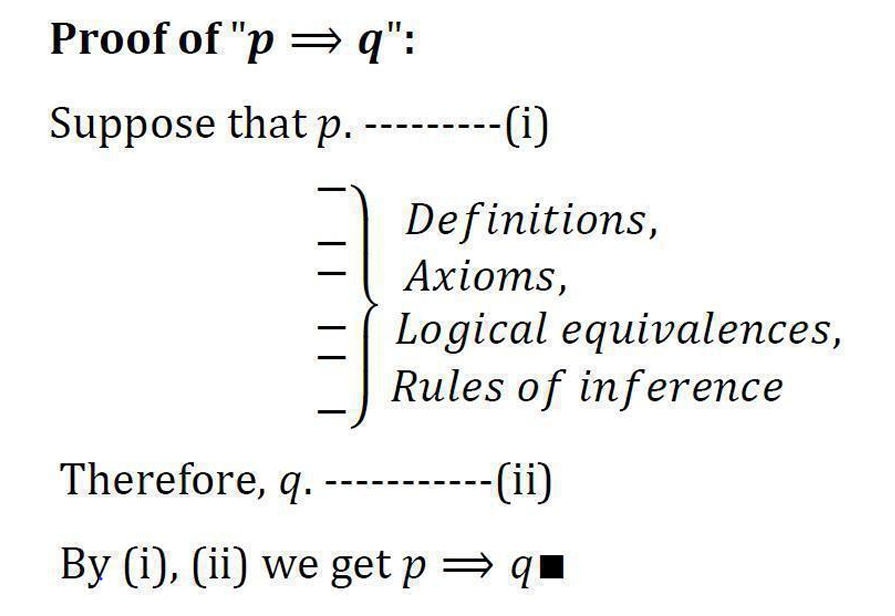
\includegraphics[width=0.6\linewidth,height=\textheight,keepaspectratio]{fig/fig3.png}

Before we begin exploring example proofs, it's essential to clearly define the foundational terms we'll be using. Based on your notes and the image provided, here are the formal definitions:

\begin{definition}[Even and Odd Integers]
\protect\hypertarget{def:unnamed-chunk-63}{}\label{def:unnamed-chunk-63}\leavevmode

\begin{itemize}
\tightlist
\item
  An integer \(n\) is \textbf{even} if there exists an integer \(k \in \mathbb{Z}\) such that:
  \[
  n = 2k
  \]
\item
  An integer \(n\) is \textbf{odd} if there exists an integer \(k \in \mathbb{Z}\) such that:
  \[
  n = 2k + 1
  \]
\item
  Every integer is either even or odd, and no integer is both.
\end{itemize}

\end{definition}

\begin{example}
\protect\hypertarget{exm:unnamed-chunk-64}{}\label{exm:unnamed-chunk-64}

\(5\) is odd integer and \(10\) is even integer.

\begin{itemize}
\tightlist
\item
  Since \(5=2\times 2 +1\)
\item
  Since \(10=2\times 5\)
\end{itemize}

\end{example}

\begin{definition}[Divisibility]
\protect\hypertarget{def:unnamed-chunk-65}{}\label{def:unnamed-chunk-65}A integer \$b \neq 0 \$ \textbf{\(b\) divides another integer \(a\)} if:
\(\exists k \in \mathbb{Z} \text{ such that } a = k \cdot b\)
** Notation**: \(b\neq 0\) divides \(a\) , written \(b \mid a\))

In this case, \(b\) is called a \textbf{factor} or \textbf{divisor} of \(a\).
\end{definition}

\begin{example}
\protect\hypertarget{exm:unnamed-chunk-66}{}\label{exm:unnamed-chunk-66}\leavevmode

\begin{itemize}
\tightlist
\item
  \(3 \mid 12\) because \(12 = 4 \cdot 3\)
\item
  \(5 \nmid 12\) because there is no integer \(k\) such that \(12 = 5k\)
\end{itemize}

\end{example}

\begin{example}
\protect\hypertarget{exm:unnamed-chunk-67}{}\label{exm:unnamed-chunk-67}Give a direct proof of the theorem ``If \(n\) is an odd integer, then \(n^2\) is odd.''
\end{example}

\begin{proof}
Let \(n \in \mathbb{Z}\) be an odd integer.\\
By definition of oddness, there exists an integer \(k \in \mathbb{Z}\) such that:
\[
n = 2k + 1
\]

Now compute \(n^2\):
\[
n^2 = (2k + 1)^2 = 4k^2 + 4k + 1 = 2(2k^2 + 2k) + 1
\]

Let \(m = 2k^2 + 2k \in \mathbb{Z}\). Then:
\[
n^2 = 2m + 1
\]

Thus, \(n^2\) is of the form \(2m + 1\), which is odd.
\end{proof}

\begin{theorem}
\protect\hypertarget{thm:unnamed-chunk-69}{}\label{thm:unnamed-chunk-69}

Let \(n\) and \(m\) be integers. Then

\begin{enumerate}
\def\labelenumi{\roman{enumi}.}
\tightlist
\item
  if \(n\) and \(m\) are both even, then \(n + m\) is even,
\item
  if \(n\) and \(m\) are both odd, then \(n + m\) is even,
\item
  if one of \(n\) and \(m\) is even and the other is odd, then \(n + m\) is odd.
\end{enumerate}

\end{theorem}

\textbf{Claim 1:} If \(n\) and \(m\) are both even, then \(n + m\) is even.

\begin{proof}
If \(n\) and \(m\) are even, then there exist integers \(a, b \in \mathbb{Z}\) such that:
\[
n = 2a,\quad m = 2b
\]
Then:
\[
n + m = 2a + 2b = 2(a + b)
\]
Since \(a + b \in \mathbb{Z}\), \(n + m\) is divisible by 2, hence even.
\end{proof}

\textbf{Claim 2:} If \(n\) and \(m\) are both odd, then \(n + m\) is even.

\begin{proof}
If \(n\) and \(m\) are odd, then there exist integers \(a, b \in \mathbb{Z}\) such that:
\[
n = 2a + 1,\quad m = 2b + 1
\]
Then:
\[
n + m = (2a + 1) + (2b + 1) = 2a + 2b + 2 = 2(a + b + 1)
\]
Since \(a + b + 1 \in \mathbb{Z}\), \(n + m\) is even.
\end{proof}

\textbf{Claim 3:} If one of \(n\) and \(m\) is even and the other is odd, then \(n + m\) is odd.

\begin{proof}
Assume without loss of generality that \(n\) is even and \(m\) is odd.\\
Then there exist integers \(a, b \in \mathbb{Z}\) such that:
\[
n = 2a,\quad m = 2b + 1
\]
Then:
\[
n + m = 2a + (2b + 1) = 2(a + b) + 1
\]
Since \(a + b \in \mathbb{Z}\), \(n + m\) is of the form \(2k + 1\), hence odd.
\end{proof}

Consider the following definitions

\begin{itemize}
\tightlist
\item
  A integer\(a \in \mathbb{Z}\). said to be Type 0: if there exist integr \(n\) such that \(a = 3n\).
\item
  A integer\(a \in \mathbb{Z}\). said to be Type 1: if there exist integr \(n\) such that \(a = 3n+1\).
\item
  A integer\(a \in \mathbb{Z}\). said to be Type 2: if there exist integr \(n\) such that \(a = 3n+2\).
\end{itemize}

\begin{enumerate}
\def\labelenumi{(\roman{enumi})}
\tightlist
\item
  If \(a\) and \(b\) are both type 1 integers, then \(a + b\) is a type 2 integer.
\end{enumerate}

\begin{proof}
Let \(a = 3m + 1\) and \(b = 3n + 1\) for some \(m, n \in \mathbb{Z}\).\\
Then:
\[
a + b = (3m + 1) + (3n + 1) = 3(m + n) + 2
\]
So \(a + b\) is of the form \(3k + 2\), hence type 2.
\end{proof}

\begin{enumerate}
\def\labelenumi{(\roman{enumi})}
\setcounter{enumi}{1}
\tightlist
\item
  If \(a\) and \(b\) are both type 2 integers, then \(a + b\) is a type 1 integer.
\end{enumerate}

\begin{proof}
Let \(a = 3m + 2\) and \(b = 3n + 2\) for some \(m, n \in \mathbb{Z}\).\\
Then:
\[
a + b = (3m + 2) + (3n + 2) = 3(m + n) + 4 = 3(m + n + 1) + 1
\]
So \(a + b\) is of the form \(3k + 1\), hence type 1.
\end{proof}

\begin{enumerate}
\def\labelenumi{(\roman{enumi})}
\setcounter{enumi}{2}
\tightlist
\item
  If \(a\) is type 1 and \(b\) is type 2, then \(ab\) is type 2.
\end{enumerate}

\begin{proof}
Let \(a = 3m + 1\), \(b = 3n + 2\) for some \(m, n \in \mathbb{Z}\).\\
Then:
\[
ab = (3m + 1)(3n + 2) = 9mn + 6m + 3n + 2 = 3(3mn + 2m + n) + 2
\]
So \(ab\) is of the form \(3k + 2\), hence type 2.
\end{proof}

\textbf{NOte}:\\
- Many logical theorems take the form:\\
\[
  \forall x (P(x) \Rightarrow Q(x))
  \]

\begin{enumerate}
\def\labelenumi{\arabic{enumi}.}
\item
  \textbf{Choose an Arbitrary Element}:\\
  Let \(c\) be an arbitrary element from the domain.
\item
  \textbf{Prove the Implication for \(c\)}:\\
  Show that \(P(c) \Rightarrow Q(c)\) holds.
\item
  \textbf{Apply Universal Generalization}:\\
  Since \(c\) was arbitrary, we conclude:\\
  \[
  \forall x (P(x) \Rightarrow Q(x))
  \]
\item
  \textbf{Focus of the Proof}:\\
  The core task is to prove a statement of the form:\\
  \[
  p \Rightarrow q
  \]
\end{enumerate}

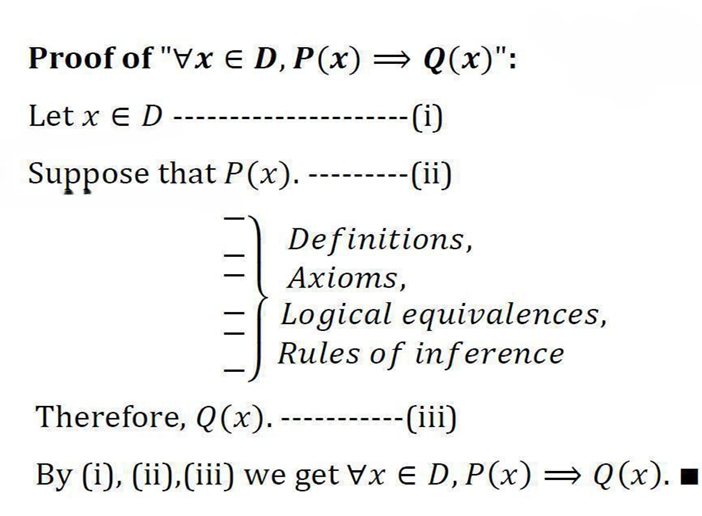
\includegraphics[width=0.6\linewidth,height=\textheight,keepaspectratio]{fig/fig4.png}
::: \{.example \#unnamed-chunk-76\}
Prove that for all \$n \in \mathbb{N} , if \(n\) is even, then \(n^2\) is even.\\
i.e.~Prove that '' \(\forall n \in  \mathbb{N}, n\) is even is even.''
:::

\begin{proof}
Let \(n \in \mathbb{N}\).\\
Suppose \(n\) is even.\\
By definition of evenness, there exists an integer \(k \in \mathbb{N}\) such that:\(n = 2k\)

Now,
\[
n^2 = (2k)^2 = 4k^2 = 2(2k^2)
\]

Since \(2k^2 \in \mathbb{N}\), it follows that \(n^2\) is divisible by 2, hence even.
\end{proof}

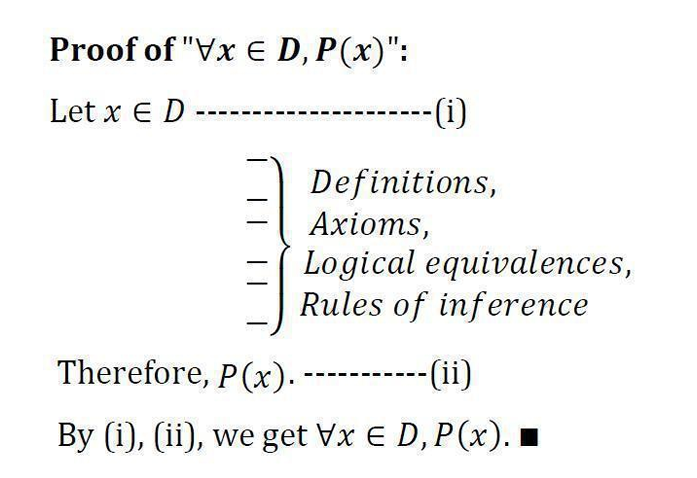
\includegraphics[width=0.6\linewidth,height=\textheight,keepaspectratio]{fig/fig5.png}

\begin{example}
\protect\hypertarget{exm:unnamed-chunk-78}{}\label{exm:unnamed-chunk-78}Prove that \(x^2 + 6x + 10 > 0\), where \(x\) is a real number.\\
We need to proove that : \(\forall x \in \mathbb{R},x^2 + 6x + 10 > 0\)
\end{example}

\begin{proof}
Let \(x\in \mathbb{R}\).\\
First note that \(x^2 + 6x + 10 = (x + 3)^2 + 1\)
\[
\begin{align}
(x+3)^2 & \geq 0\\
(x+3)^2+1 & \geq 1>0
\end{align}
\]

Threfore, \(\forall x \in \mathbb{R},x^2 + 6x + 10 > 0\)
\end{proof}

\subsection{Proof by Contradiction}\label{proof-by-contradiction}

Given a statement \(p\), assume it is false.\\
Assume\(\neg p\).\\
Prove that \(\neg p\) leads to false.\\
A contradiction exists.\\

\begin{itemize}
\tightlist
\item
  Given a statement of the form \(p \implies q\).
  To assume it's false, you only have to consider the case where \(p\) is true and \(q\) is false.
\end{itemize}

\pandocbounded{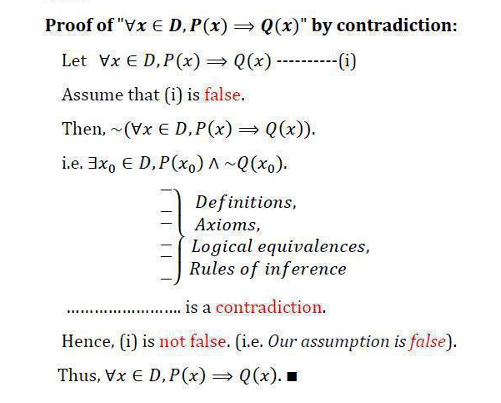
\includegraphics[keepaspectratio]{fig/fig6.png}}

\textbf{Claim:} If \(n^2\) is even, then \(n\) is even.

\pandocbounded{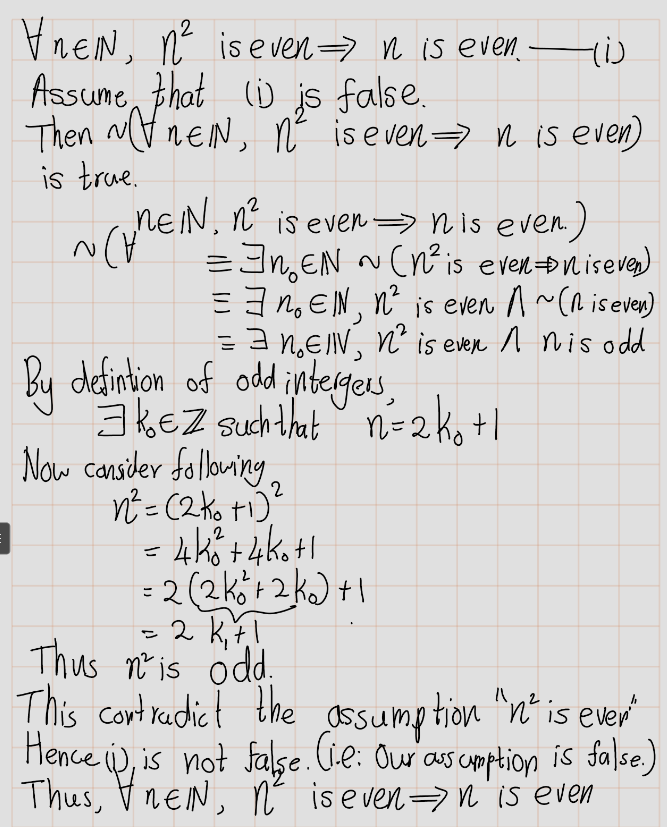
\includegraphics[keepaspectratio]{fig/fig7.png}}

\begin{example}
\protect\hypertarget{exm:unnamed-chunk-80}{}\label{exm:unnamed-chunk-80}Prove: \(\forall  x \in \mathbb{R}, x^2 + 6x + 10 > 0\)
\end{example}

\begin{proof}
Suppose that
begin\{equation\}
\forall  x \in \mathbb{R}, x\^{}2 + 6x + 10 \textgreater{} 0 \label{eq:eq5}
\textbackslash end\{equation\}
Assume that statement \eqref{eq:eq5} is false. ~
\(x_0^2 + 6x_0 + 10 \leq 0\) for some \(x_0 \in \mathbb{R})\).\\
Now \(x_0^2 + 6x_0 + 10 =(x_0+3)^2+1\geq 1\).\\
Hence, \(0<1\leq 0\). This is a contradiction.\\
\(\therefore\) \eqref{eq:eq5} is false.\\
\(\forall  x \in \mathbb{R}, x^2 + 6x + 10 > 0\)
\end{proof}

\begin{exercise}
\protect\hypertarget{exr:unnamed-chunk-82}{}\label{exr:unnamed-chunk-82}\textbf{Claim:} If \(n = ab\), then \(a \leq \sqrt{n}\) or \(b \leq \sqrt{n}\), where \(a, b \in \mathbb{Z}^+\).\\
\(\exists x_0 \in \mathbb{R}\) such that \(x_0^2 + 6x_0 + 10 \leq 0\).
\end{exercise}

\begin{exercise}
\protect\hypertarget{exr:unnamed-chunk-83}{}\label{exr:unnamed-chunk-83}\textbf{Claim:} \(\sqrt{2} \notin \mathbb{Q}\), where \(\mathbb{Q}=\left\{\frac{p}{q}:p,q \in \mathbb{Z}, q\neq 0\right\}\)
\end{exercise}

\section{Indirect Proofs}\label{indirect-proofs}

Consider an implication:

\[
p \Rightarrow q
\]

Its contrapositive is:

\[
\neg q \Rightarrow \neg p
\]

This contrapositive is logically equivalent to the original implication.\\
Thus, to prove \(p \Rightarrow q\), we may instead prove \(\neg q \Rightarrow \neg p\).

To perform an \textbf{indirect proof}, carry out a \textbf{direct proof} on the contrapositive.

\begin{example}
\protect\hypertarget{exm:unnamed-chunk-84}{}\label{exm:unnamed-chunk-84}Prove that: If \(x^2\) is even, then \(x\) is even.
\end{example}

\begin{example}
\protect\hypertarget{exm:unnamed-chunk-85}{}\label{exm:unnamed-chunk-85}Prove that: If \((x - 2)^2 \neq 1\), then \(x \neq 3\)
\end{example}

\section{Proof by Cases}\label{proof-by-cases}

\begin{example}
\protect\hypertarget{exm:unnamed-chunk-86}{}\label{exm:unnamed-chunk-86}Let \(x\) be any integer. Then \(x^2 + x\) is even.
\end{example}

To prove: \(\exists x \in \mathbb{Z},\; P(x)\)

We exhibit a member of the universal set for which \(P(x)\) is true.\\
One example suffices.

\begin{example}
\protect\hypertarget{exm:unnamed-chunk-87}{}\label{exm:unnamed-chunk-87}Show that:

\[
\exists x \in \mathbb{Z} \text{ such that } x^2 = 4
\]
\end{example}

\begin{proof}
Let \(x_0 = -2\). Then:
- \(x_0 \in \mathbb{Z}\)
- \(x_0^2 = (-2)^2 = 4\)

Thus, \(\exists x_0 \in \mathbb{Z},\quad x_0^2 = 4\)
\end{proof}

\section{Proof by Principle of Mathematical Induction}\label{proof-by-principle-of-mathematical-induction}

\subsection{Principle of Mathematical Induction}\label{principle-of-mathematical-induction}

Let \(P(n)\) be a statement defined for each positive integer \(n \in \mathbb{N}\).\\
To prove that \(P(n)\) is true for all \(n \in \mathbb{N}\), it suffices to show:

\begin{enumerate}
\def\labelenumi{\arabic{enumi}.}
\item
  \textbf{Base Case}:\\
  \(P(1)\) is true.
\item
  \textbf{Inductive Step}:\\
  For every \(k \in \mathbb{N}\), if \(P(k)\) is true, then \(P(k+1)\) is also true.\\
  That is:
  \[   \forall k \in \mathbb{N},\; P(k) \Rightarrow P(k+1)\]
\item
  \textbf{Conclusion}: If both the base case and the inductive step are established, then:
  \[
  \forall n \in \mathbb{N},\; P(n) \text{ is true}
  \]
\end{enumerate}

This is the foundation for proving propositions over the natural numbers.

\begin{example}
\protect\hypertarget{exm:unnamed-chunk-89}{}\label{exm:unnamed-chunk-89}Prove by induction that\\
\[
1 + 2 + 3 + \cdots + n = \frac{n(n+1)}{2}
\quad \text{for all } n \in \mathbb{N}.
\]
\end{example}

\begin{example}
\protect\hypertarget{exm:unnamed-chunk-90}{}\label{exm:unnamed-chunk-90}Prove by induction that\\
\[
n^3 + 2n \text{ is divisible by } 3
\quad \text{for all } n \in \mathbb{N}.
\]
\end{example}

\section{Exercises}\label{exercises}

\begin{exercise}
\protect\hypertarget{exr:unnamed-chunk-91}{}\label{exr:unnamed-chunk-91}Prove by induction that\\
\[
2^{n+1} > n^2
\quad \text{for all } n \in \mathbb{N}.
\]
\end{exercise}

\begin{exercise}
\protect\hypertarget{exr:unnamed-chunk-92}{}\label{exr:unnamed-chunk-92}

Let the sequence \((a_n)\) be defined recursively by\\
\[
a_1 = \sqrt{2}, \quad a_{n+1} = \sqrt{2 + a_n}, \quad \text{for all } n \in \mathbb{N}.
\]

Prove the following properties:

\begin{enumerate}
\def\labelenumi{(\alph{enumi})}
\tightlist
\item
  \(a_n > 0\) for all \(n \in \mathbb{N}\).\\
\item
  \(a_n \leq 2\) for all \(n \in \mathbb{N}\).\\
\item
  \(a_{n+1} \geq a_n\) for all \(n \in \mathbb{N}\).
\end{enumerate}

\end{exercise}

\chapter{\texorpdfstring{The Real Number System \(\mathbb{R}\)}{The Real Number System \textbackslash mathbb\{R\}}}\label{the-real-number-system-mathbbr}

\subsection{Topics Covered}\label{topics-covered}

\begin{itemize}
\tightlist
\item
  Axioms of Real Numbers\\
\item
  Order Axioms and Axiom of Bounds\\
\item
  Supremum and Infimum of Subsets of \(\mathbb{R}\)\\
\item
  Concept of Infinity and Intervals of \(\mathbb{R}\)
\end{itemize}

\subsection{What Are the Real Numbers?}\label{what-are-the-real-numbers}

The question ``What are the real numbers?'' is, for now, too deep to answer directly. Instead, we adopt a formal approach: we assume the existence of a set \(\mathbb{R}\), called the set of real numbers, and impose a collection of axioms that define its structure.

All subsequent mathematical development will be based solely on these axioms.

\section{Axioms of real numbers}\label{axioms-of-real-numbers}

We assume that there are two binary operations on \(\mathbb{R}\), that is, ``\(+\)'' and ``\(\cdot\)'' the first called \textbf{addition}, and second \textbf{multiplication}, such that \(a + b \in \mathbb{R}\) and \(a\cdot b \in \mathbb{R}\) for all \(a, b \in \mathbb{R}\), and the following properties are satisfied:

\textbf{A1. Commutativity of Addition}\\
For all \(a, b \in \mathbb{R}\), .\(a + b = b + a\)

\textbf{A2. Associativity of Addition}\\
For all \(a, b, c \in \mathbb{R}\), \(a + (b + c) = (a + b) + c\)

\textbf{A3. Existence of Additive Identity}\\
There exists an element \(0 \in \mathbb{R}\) such that for all \(a \in \mathbb{R}\), \(a + 0 = a\)

\textbf{A4. Existence of Additive Inverse}\\
For every \(a \in \mathbb{R}\), there exists an element \(-a \in \mathbb{R}\) such that: \(a + (-a) = 0\)

\textbf{A5. Commutativity of Multiplication}\\
For all \(a, b \in \mathbb{R}\), \(a \cdot b = b \cdot a\)

\textbf{A6. Associativity of Multiplication}\\
For all \(a, b, c \in \mathbb{R}\), \(a \cdot (b \cdot c) = (a \cdot b) \cdot c\)

\textbf{A7. Existence of Multiplicative Identity}\\
There exists an element \(1 \in \mathbb{R}\) such that for all \(a \in \mathbb{R}\), \(a \cdot 1 = a\)

\textbf{A8. Existence of Multiplicative Inverse}\\
For every \(a \in \mathbb{R}\) with \(a \ne 0\), there exists an element \(a^{-1} \in \mathbb{R}\) such that: \(a \cdot a^{-1} = 1\)

\textbf{A9. Distributivity of Multiplication over Addition}\\
For all \(a, b, c \in \mathbb{R}\),\(a \cdot (b + c) = a \cdot b + a \cdot c\)

Thank you, Ashan. Based on your image, here's a formal Markdown rendering of the \textbf{Basic Properties of Equality} and \textbf{Some Algebraic Properties of Real Numbers}, using LaTeX for clarity and textbook precision:

\section{Basic Properties of Equality}\label{basic-properties-of-equality}

Let \(x, y, z \in \mathbb{R}\). Then:

\begin{enumerate}
\def\labelenumi{\arabic{enumi}.}
\item
  \textbf{Reflexivity}:\\
  \[
  x = x
  \]
\item
  \textbf{Symmetry}:\\
  If \(x = y\), then \(y = x\).
\item
  \textbf{Transitivity}:\\
  If \(x = y\) and \(y = z\), then \(x = z\).
\end{enumerate}

\section{Some Algebraic Properties of Real Numbers}\label{some-algebraic-properties-of-real-numbers}

Let \(a, b, c \in \mathbb{R}\). Then:

\begin{enumerate}
\def\labelenumi{\roman{enumi}.}
\item
  \textbf{Cancellation Law for Addition}:\\
  If \(a + b = a + c\), then \(b = c\).
\item
  \textbf{Multiplication by Zero}:\\
  \[
     a \cdot 0 = 0
     \]
\item
  \textbf{Zero Product Property}:\\
  If \(a \cdot b = 0\), then \(a = 0\) or \(b = 0\).
\end{enumerate}

\begin{proof}
\leavevmode

.\\

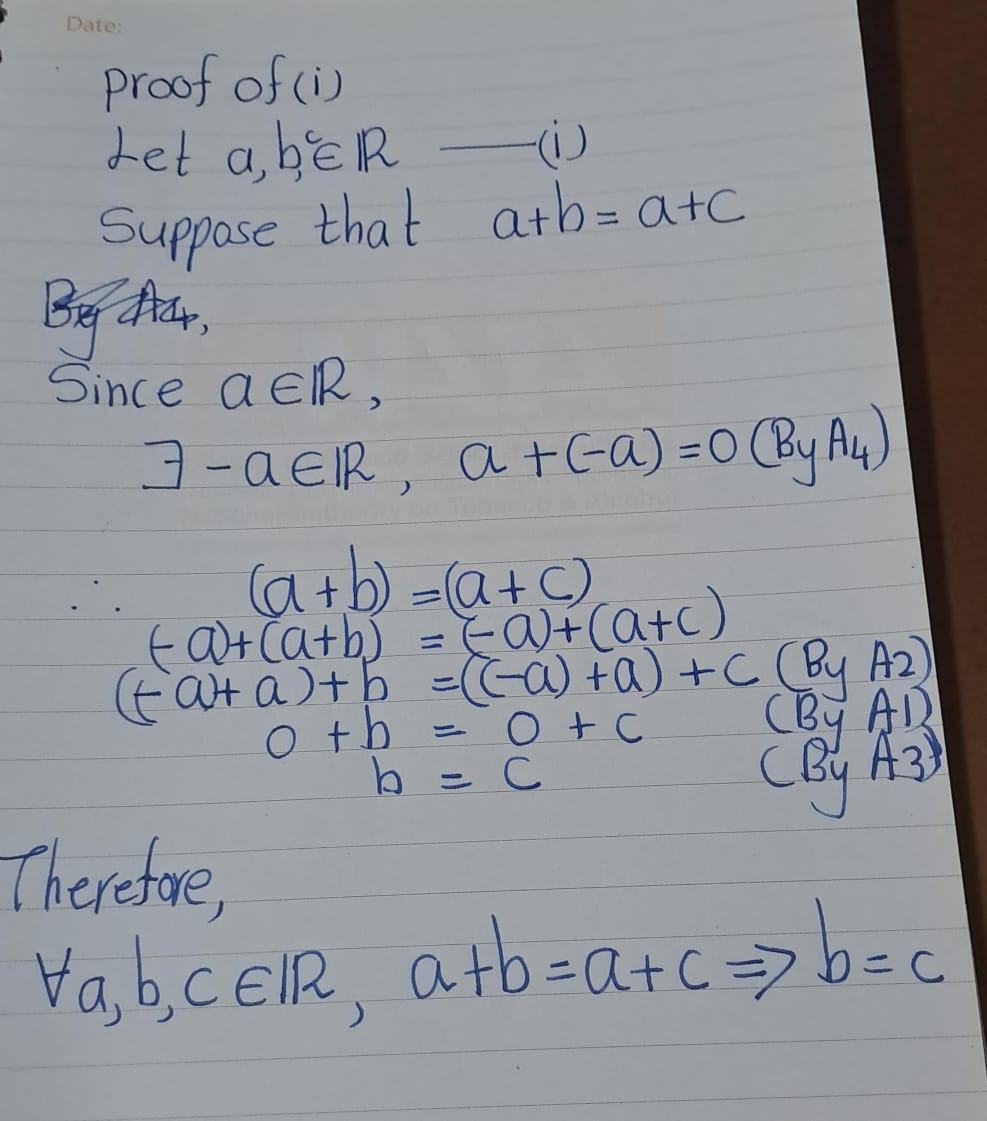
\includegraphics[width=0.8\linewidth,height=\textheight,keepaspectratio]{fig/fig8.jpg}

rest of them leave as an exercise

\end{proof}

\subsection{Selected Theorems}\label{selected-theorems}

These theorems follow from the axioms of the real numbers. In all cases, \(a, b, c, d \in \mathbb{R}\), with additional nonzero conditions where specified.

\begin{enumerate}
\def\labelenumi{\arabic{enumi}.}
\item
  Properties of Zero

  \begin{enumerate}
  \def\labelenumii{\alph{enumii}.}
  \tightlist
  \item
    \(a - a = 0\)
  \item
    \(0 = -a + a\)
  \item
    \(0 \cdot a = 0\)
  \item
    If \(ab = 0\), then \(a = 0\) or \(b = 0\)
  \end{enumerate}
\item
  Properties of Signs

  \begin{enumerate}
  \def\labelenumii{\alph{enumii}.}
  \tightlist
  \item
    \(-0 = 0\)
  \item
    \(-(-a) = a\)
  \item
    \((-a)b = -(ab) = a(-b)\)
  \item
    \((-a)(-b) = ab\)
  \item
    \(-a = (-1)a\)
  \end{enumerate}
\item
  Additional Distributive Properties

  \begin{enumerate}
  \def\labelenumii{\alph{enumii}.}
  \tightlist
  \item
    \(-(a + b) = -a - b\)
  \item
    \(a - b = -(b - a)\)
  \item
    \(-(a - b) = b - a\)
  \item
    \(a + a = 2a\)
  \item
    \(a(b - c) = ab - ac = (b - c)a\)
  \item
    \((a + b)(c + d) = ac + ad + bc + bd\)
  \item
    \((a + b)(c - d) = ac - ad + bc - bd = (c - d)(a + b)\)
  \item
    \((a - b)(c - d) = ac - ad - bc + bd\)
  \end{enumerate}
\item
  Properties of Inverses (for \(a, b \ne 0\))

  \begin{enumerate}
  \def\labelenumii{\alph{enumii}.}
  \tightlist
  \item
    If \(a \ne 0\), then \(a^{-1} \ne 0\)
  \item
    \(1^{-1} = 1\)
  \item
    \((a^{-1})^{-1} = a\)
  \item
    \((-a)^{-1} = -(a^{-1})\)
  \item
    \((ab)^{-1} = a^{-1}b^{-1}\)
  \item
    \(\left( \frac{a}{b} \right)^{-1} = \frac{b}{a}\)
  \end{enumerate}
\item
  Properties of Quotients (for nonzero denominators)

  \begin{enumerate}
  \def\labelenumii{\alph{enumii}.}
  \tightlist
  \item
    \(\frac{a}{1} = a\)
  \item
    \(\frac{1}{a} = a^{-1}\)
  \item
    \(\frac{a}{a} = 1\)
  \item
    \(\frac{a/b}{c/d} = \frac{ac}{bd}\)
  \item
    \(\frac{a/b}{c/d} = \frac{ad}{bc}\)
  \item
    \(\frac{ac}{bc} = \frac{a}{b}\)
  \item
    \(\frac{a}{b/c} = \frac{ab}{c}\)
  \item
    \(\frac{ab}{b} = a\)
  \item
    \(\frac{-a}{b} = -\left( \frac{a}{b} \right) = \frac{a}{-b}\)
  \item
    \(\frac{-a}{-b} = \frac{a}{b}\)
  \item
    \(\frac{a}{b} + \frac{c}{d} = \frac{ad + bc}{bd}\)
  \item
    \(\frac{a}{b} - \frac{c}{d} = \frac{ad - bc}{bd}\)
  \end{enumerate}
\end{enumerate}

\begin{exercise}
\protect\hypertarget{exr:unnamed-chunk-94}{}\label{exr:unnamed-chunk-94}Proove theroms
\end{exercise}

\section{The Order Axioms and Axiom of Bounds}\label{the-order-axioms-and-axiom-of-bounds}

We assume the existence of a subset \(P \subseteq \mathbb{R}\) with the following properties:

\textbf{A10.} For any \(a \in \mathbb{R}\), exactly one of the following holds:
\(a \in P \text{ or }  a = 0 \text{ or } -a \in P\)

\textbf{A11.} If \(a, b \in P\), then \(a + b \in P\) and \(a \cdot b \in P\)

\begin{definition}
\protect\hypertarget{def:unnamed-chunk-95}{}\label{def:unnamed-chunk-95}For any \(a, b \in \mathbb{R}\), we define:
\[
a > b \quad \text{if and only if} \quad a - b \in P
\]

Equivalently, \(b < a\).
\end{definition}

\textbf{Note}: Axioms A10 and A11, together with Axioms A1--A9, endow the field \((\mathbb{R}, +, \cdot)\) with an order structure.\\
Thus, \(\mathbb{R}\) becomes an \textbf{ordered field}.

\begin{exercise}
\protect\hypertarget{exr:unnamed-chunk-96}{}\label{exr:unnamed-chunk-96}Prove that for all \(a \in P\), we have \(a > 0\).
\end{exercise}

\begin{exercise}
\protect\hypertarget{exr:unnamed-chunk-97}{}\label{exr:unnamed-chunk-97}Prove that \(1 \in P\), i.e., \(1 > 0\).
\end{exercise}

\begin{exercise}
\protect\hypertarget{exr:unnamed-chunk-98}{}\label{exr:unnamed-chunk-98}Prove that if \(a > 0\), then \(x_a > 0\) for all \(a \in \mathbb{R}\).
\end{exercise}

\begin{theorem}
\protect\hypertarget{thm:unnamed-chunk-99}{}\label{thm:unnamed-chunk-99}For any two real numbers \(a, b\), exactly one of the following holds:
- \(a < b \text{ or } b < a \text{ or } a = b\)
\end{theorem}

\begin{theorem}[Order Properties of Real Numbers]
\protect\hypertarget{thm:unnamed-chunk-100}{}\label{thm:unnamed-chunk-100}

Let \(a, b, c \in \mathbb{R}\). Then:

\begin{enumerate}
\def\labelenumi{\arabic{enumi}.}
\item
  \textbf{Transitivity}\\
  If \(a < b\) and \(b < c\), then \(a < c\).
\item
  \textbf{Addition Preservation}\\
  If \(a < b\), then \(a + c < b + c\).
\item
  \textbf{Multiplication by Positive}\\
  If \(c > 0\) and \(a < b\), then \(a \cdot c < b \cdot c\).
\item
  \textbf{Multiplication by Negative}\\
  If \(c < 0\) and \(a < b\), then \(a \cdot c > b \cdot c\).\\
  \emph{(Note: This reverses the inequality.)}
\end{enumerate}

\end{theorem}

Thanks, Ashan. Here's a formal transcription of the image content, formatted for textbook inclusion:

\begin{center}\rule{0.5\linewidth}{0.5pt}\end{center}

\section{Absolute Value}\label{absolute-value}

\begin{definition}
\protect\hypertarget{def:unnamed-chunk-101}{}\label{def:unnamed-chunk-101}For any real number \(x\), the absolute value (or modulus) of \(x\) is defined as:
\[
|x| = 
\begin{cases}
x, & \text{if } x \geq 0 \\
-x, & \text{if } x < 0
\end{cases}
\]
\end{definition}

\begin{theorem}[Properties of Absolute Value]
\protect\hypertarget{thm:unnamed-chunk-102}{}\label{thm:unnamed-chunk-102}

Let \(a, b \in \mathbb{R}\). Then:

\begin{enumerate}
\def\labelenumi{\arabic{enumi}.}
\tightlist
\item
  \(|a| = 0 \iff a = 0\)
\item
  \(|a| \geq 0\)
\item
  \(|a| = |-a|\)
\item
  \(-|a| \leq a \leq |a|\)
\item
  If \(b > 0\), then \(|a| \leq b \iff -b \leq a \leq b\)
\item
  If \(b > 0\), then \(|a| \geq b \iff a \geq b\) or \(a \leq -b\)
\item
  \(|a + b| \leq |a| + |b|\)
\end{enumerate}

\end{theorem}

\emph{Proof}: Leave as a exercise

\begin{example}
\protect\hypertarget{exm:unnamed-chunk-103}{}\label{exm:unnamed-chunk-103}\leavevmode

\begin{enumerate}
\def\labelenumi{\arabic{enumi}.}
\tightlist
\item
  If \(a < b\) and both \(a, b > 0\), then \(a^{-1} > b^{-1}\).
\item
  \(ab > 0 \iff a, b\) are both positive or both negative.
\item
  \(ab < 0 \iff\) one of \(a, b\) is positive and the other is negative.
\end{enumerate}

\end{example}

\begin{definition}[Minimum and Maximum]
\protect\hypertarget{def:unnamed-chunk-104}{}\label{def:unnamed-chunk-104}

Let \(A \subseteq \mathbb{R}\) be a non-empty set.

\begin{itemize}
\item
  An element \(m \in A\) is called the \textbf{minimum} of \(A\) if:\(m \leq x \quad \text{for all } x \in A\)
\item
  An element \(M \in A\) is called the \textbf{maximum} of \(A\) if:\(M \geq x \quad \text{for all } x \in A\)
\end{itemize}

\end{definition}

\textbf{Note:} If a minimum or maximum exists, it is unique.

\begin{example}
\protect\hypertarget{exm:unnamed-chunk-105}{}\label{exm:unnamed-chunk-105}

Let \(A = \{2, -3, 8, 17, -5\}\)

\begin{itemize}
\item
  \textbf{Minimum of \(A\)}:\\
  \(\min A = -5\). (Because \(2 \geq -5,
  -3\geq -5,
  8 \geq -5,
  17\geq -5,
  -5 \geq -5\)).
\item
  \textbf{Maximum of \(A\)}:\\
  \(\max A = 17\). (Because \(2 \leq 17,
  -3\leq 17,
  8 \leq 17,
  17\leq 17,
  -5 \leq 17\))
\end{itemize}

\end{example}

\begin{example}
\protect\hypertarget{exm:unnamed-chunk-106}{}\label{exm:unnamed-chunk-106}Let \(A = \{1 + \frac{2}{n} \mid n \in \mathbb{N} \}\)

This is an infinite set of real numbers:
\[
A = \left\{1 + \frac{2}{1}, 1 + \frac{2}{2}, 1 + \frac{2}{3}, \dots \right\} = \left\{3, 2, \frac{5}{3}, \dots \right\}
\]
\end{example}

\begin{definition}[Bounded Above]
\protect\hypertarget{def:unnamed-chunk-107}{}\label{def:unnamed-chunk-107}A non-empty set \(A \subseteq \mathbb{R}\) is said to be \textbf{bounded above} if there exists a number \(k \in \mathbb{R}\) such that:\(\forall x \in A, \quad x \leq k\)

The number \(k\) is called an \textbf{upper bound} of the set \(A\).
\end{definition}

\begin{definition}[Bounded Below]
\protect\hypertarget{def:unnamed-chunk-108}{}\label{def:unnamed-chunk-108}A non-empty set \(A \subseteq \mathbb{R}\) is said to be \textbf{bounded below} if there exists a number \(k \in \mathbb{R}\) such that:

\[
\forall x \in A, \quad x \geq k
\]

The number \(k\) is called a \textbf{lower bound} of the set \(A\).
\end{definition}

\textbf{Note:}
Let \(M \subseteq d\) and \(A \subseteq \mathbb{R}\).

\begin{itemize}
\item
  A set \(A\) is bounded above \(\underbrace{\iff}_{\text{Def}^\text{n}}
  \exists k \in \mathbb{R} \quad \forall x \in A, \quad x \leq k\)
\item
  A set \(A\) is \textbf{not} bounded above \(\iff \neg (\exists k \in \mathbb{R} \quad \forall x \in A, \quad x \leq k)\equiv\forall k \in \mathbb{R} \quad \exists x \in A, \quad x > k\)
\end{itemize}

\begin{example}
\protect\hypertarget{exm:unnamed-chunk-109}{}\label{exm:unnamed-chunk-109}Let \(A = \{ x \in \mathbb{R} \mid x \geq -7 \}\) and \(B = \{ 2n + 3 \mid n \in \mathbb{N} \}\)
\end{example}

\textbf{Note:}
Let \(M \subseteq d\) and \(A \subseteq \mathbb{R}\).

\begin{itemize}
\item
  A set \(A\) is bounded below \(\underbrace{\iff}_{\text{Def}^\text{n}}
  \exists k \in \mathbb{R} \quad \forall x \in A, \quad x \geq k\)
\item
  A set \(A\) is \textbf{not} bounded below \(\iff \neg (\exists k \in \mathbb{R} \quad \forall x \in A, \quad x \geq k)\equiv\forall k \in \mathbb{R} \quad \exists x \in A, \quad x > k\)
\end{itemize}

\begin{definition}
\protect\hypertarget{def:unnamed-chunk-110}{}\label{def:unnamed-chunk-110}

Let \(A \subseteq \mathbb{R}\), with \(A \neq \emptyset\).

\begin{itemize}
\tightlist
\item
  A set \(A\) is \textbf{bounded} if it is both bounded above and bounded below.
\item
  A set \(A\) is \textbf{unbounded} if it is not bounded.
\end{itemize}

\end{definition}

\begin{definition}[Least Upper Bound (Supremum)]
\protect\hypertarget{def:unnamed-chunk-111}{}\label{def:unnamed-chunk-111}

An element \(\lambda \in \mathbb{R}\) is called the \textbf{least upper bound} (or \textbf{supremum}) of \(A\) if:

\begin{enumerate}
\def\labelenumi{\arabic{enumi}.}
\tightlist
\item
  \(\lambda\) is an upper bound of \(A\), i.e.,
  \[
  \forall x \in A, \quad x \leq \lambda
  \]
\item
  No upper bound of \(A\) is less than \(\lambda\), i.e.,
  \[
  \forall u \in \mathbb{R}, \left( \forall x \in A, \ x \leq u \right) \Rightarrow \lambda \leq u
  \]
\end{enumerate}

\end{definition}

\begin{definition}[Greatest Lower Bound (Infimum)]
\protect\hypertarget{def:unnamed-chunk-112}{}\label{def:unnamed-chunk-112}

An element \(\mu \in \mathbb{R}\) is called the \textbf{greatest lower bound} (or \textbf{infimum}) of \(A\) if:

\begin{enumerate}
\def\labelenumi{\arabic{enumi}.}
\tightlist
\item
  \(\mu\) is a lower bound of \(A\), i.e.,
  \[
  \forall x \in A, \quad x \geq \mu
  \]
\item
  No lower bound of \(A\) is greater than \(\mu\), i.e.,
  \[
  \forall u \in \mathbb{R}, \left( \forall x \in A, \ x \geq u \right) \Rightarrow \mu \geq u
  \]
\end{enumerate}

\end{definition}

\section{Axiom of Bound (Completeness Axiom)}\label{axiom-of-bound-completeness-axiom}

\textbf{A12. Least Upper Bound Axiom}

If \(A \subseteq \mathbb{R}\) is non-empty and bounded above, then:

\[
\exists \sup A \in \mathbb{R}
\]

That is, every non-empty subset of \(\mathbb{R}\) that is bounded above has a \textbf{least upper bound} (supremum) in \(\mathbb{R}\).

\textbf{A12′. Greatest Lower Bound Axiom}

If \(A \subseteq \mathbb{R}\) is non-empty and bounded below, then:

\[
\exists \inf A \in \mathbb{R}
\]

That is, every non-empty subset of \(\mathbb{R}\) that is bounded below has a \textbf{greatest lower bound} (infimum) in \(\mathbb{R}\).

\begin{example}
\protect\hypertarget{exm:unnamed-chunk-113}{}\label{exm:unnamed-chunk-113}Let \(A = \{ x \in \mathbb{R} \mid x^2 < 2 \}\)

\begin{itemize}
\tightlist
\item
  This set is \textbf{bounded above}.
\item
  The least upper bound (supremum) of \(A\) is:
\end{itemize}

\[
\sup A = \lambda
\]

Since:

\[
\sqrt{2}^2 = 2 \quad \text{and} \quad \sqrt{2} \in \mathbb{R}
\]
\end{example}

Thank you for sharing the image. Here's a formal Markdown transcription using LaTeX notation, suitable for textbook inclusion:

\begin{center}\rule{0.5\linewidth}{0.5pt}\end{center}

\section{Archimedean Property}\label{archimedean-property}

\begin{theorem}[Archimedean Property]
\protect\hypertarget{thm:unnamed-chunk-114}{}\label{thm:unnamed-chunk-114}For all \(a \in \mathbb{R}^+\) and \(b \in \mathbb{R}\), there exists \(n \in \mathbb{N}\) such that: \(na \geq b\)
\end{theorem}

\begin{proof}
Suppose the Archimedean Property is false.
Then\(\exists a \in \mathbb{R}^+, \exists b \in \mathbb{R}, \forall n \in \mathbb{N}, \quad na \leq b\)

Define the set \(S := \{ na \mid n \in \mathbb{N} \}\)

Then \(b\) is an upper bound of \(S\). By the completeness axiom, the supremum \(s_0 := \sup S\) exists.

Let \(n \in \mathbb{N}\). Then \(n + 1 \in \mathbb{N}\), and \(s_0 \geq (n + 1)a = na + a \Rightarrow s_0 - a \geq na\)

So \(s_0 - a\) is an upper bound of \(S\), but \(s_0 - a < s_0\)

This contradicts the fact that \(s_0\) is the least upper bound of \(S\). Hence, the Archimedean Property holds. 
\end{proof}

\begin{corollary}
\protect\hypertarget{cor:unnamed-chunk-116}{}\label{cor:unnamed-chunk-116}For any \(x \in \mathbb{R}\) with \(x > 0\), there exists \(n \in \mathbb{N}\) such that \(\frac{1}{n} < x\)
\end{corollary}

\begin{proof}
Let \(a = x\), \(b = 1\). Since \(a > 0\), by the Archimedean Property, there exists \(n \in \mathbb{N}\) such that:

\[
na > 1 \Rightarrow x > \frac{1}{n}
\]
\end{proof}

\section{\texorpdfstring{Concept of Infinity and Intervals of \(\mathbb{R}\)}{Concept of Infinity and Intervals of \textbackslash mathbb\{R\}}}\label{concept-of-infinity-and-intervals-of-mathbbr}

\subsection{Concept of Infinity}\label{concept-of-infinity}

\begin{figure}
\centering
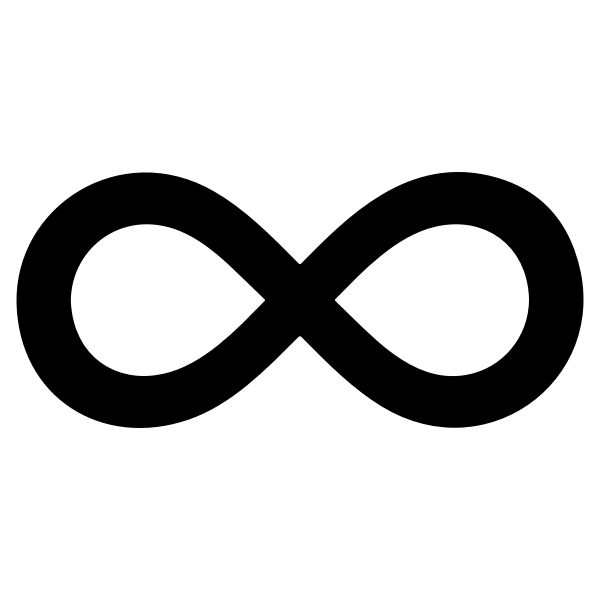
\includegraphics[width=0.2\linewidth,height=\textheight,keepaspectratio]{fig/fig8.png}
\caption{The infinity symbol is a mathematical symbol representing the concept of infinity. This symbol is also called a lemniscate,}
\end{figure}

Infinity comes from the Latin \emph{infinitas}, meaning ``unboundedness.'' It refers to several distinct concepts---usually linked to the idea of ``without end.''

\begin{itemize}
\tightlist
\item
  We encounter infinity for the first time in school, where we meet the set:
\end{itemize}

\[
\mathbb{N} = \{1, 2, 3, \dots\}
\]

\begin{itemize}
\tightlist
\item
  The concept of this set can be formulated as follows:
\end{itemize}

For each natural number \(n\), there exists a larger natural number \(n + 1\).\\
In other words, there does not exist a natural number that is larger than all natural numbers.\\
That is, there exists no largest natural number.

• We are unable to write down the list of all natural
numbers.
• Hence, our writing is never- ending process,
because of this we talk about infinity or
unboundedness of natural numbers.
• We realize that we have infinitely many natural
numbers, but we are unable to perceive all natural
numbers at once.
• We have a similar situation with the idea (the notion)
of a line in Geometry.
• Length of any line is infinite or unbounded
(infinitely large)
• One can walk along a line for an arbitrarily long
time and one never reaches the end.
• We unable to see a whole infinite line at once.

• The main problem with understanding the concept of
infinity is that we are not capable of imagining object
at once.
• We are only able to see a finite fraction (part) of
an infinite object.
• The way out we use is to denote infinite objects
by symbols.
• We work with these symbols as a finite
representation of the corresponding infinite
objects.
Infinity is not a number, but a concept that describes something unbounded or without limit.

\begin{itemize}
\item
  Infinity is not a number, but a concept that describes something \textbf{unbounded} or \textbf{without limit}.
\item
  In mathematics, we denote infinity using the symbol:
\end{itemize}

\[
\infty
\]

\subsection{\texorpdfstring{\textbf{Infinity in \(\mathbb{R}\)}}{Infinity in \textbackslash mathbb\{R\}}}\label{infinity-in-mathbbr}

Let \(S \subseteq \mathbb{R}\) be a non-empty subset.

\begin{itemize}
\tightlist
\item
  \(S\) is \textbf{not bounded above} if it has no upper bound.
\item
  \(S\) is \textbf{not bounded below} if it has no lower bound.
\end{itemize}

To facilitate mathematical reasoning, we adjoin two \textbf{fictitious points} to \(\mathbb{R}\):

\begin{itemize}
\tightlist
\item
  \(+\infty\) (often written simply as \(\infty\))
\item
  \(-\infty\)
\end{itemize}

These points are \textbf{not elements of} \(\mathbb{R}\), i.e.,

\[
\infty, -\infty \notin \mathbb{R}
\]

For any real number \(x \in \mathbb{R}\):

\[
-\infty < x < \infty
\]

If \(S \subseteq \mathbb{R}\) is non-empty and \textbf{not bounded above}, we write:

\[
\sup S = \infty
\]

This notation indicates that \(S\) has no finite supremum.

\subsection{\texorpdfstring{Intervals in \(\mathbb{R}\)}{Intervals in \textbackslash mathbb\{R\}}}\label{intervals-in-mathbbr}

\begin{definition}
\protect\hypertarget{def:unnamed-chunk-118}{}\label{def:unnamed-chunk-118}

Let \(a, b \in \mathbb{R}\) with \(a < b\). We define the following intervals:

\begin{itemize}
\item
  \textbf{Bounded Intervals}

  \begin{itemize}
  \item
    \textbf{Closed Interval}:
    \[
      [a, b] = \{ x \in \mathbb{R} \mid a \leq x \leq b \}
      \]
  \item
    \textbf{Open Interval}:
    \[
      (a, b) = \{ x \in \mathbb{R} \mid a < x < b \}
      \]
  \item
    \textbf{Half-Open Intervals}:
    \[
      (a, b] = \{ x \in \mathbb{R} \mid a < x \leq b \}, \quad [a, b) = \{ x \in \mathbb{R} \mid a \leq x < b \}
      \]
  \end{itemize}
\end{itemize}

These are called \textbf{bounded intervals} because both endpoints \(a\) and \(b\) are real numbers.

\begin{itemize}
\item
  \textbf{Unbounded Intervals}

  \begin{itemize}
  \item
    \textbf{Right-Unbounded}:
    \[
      [a, \infty) = \{ x \in \mathbb{R} \mid x \geq a \}, \quad (a, \infty) = \{ x \in \mathbb{R} \mid x > a \}
      \]
  \item
    \textbf{Left-Unbounded}:
    \[
      (-\infty, b] = \{ x \in \mathbb{R} \mid x \leq b \}, \quad (-\infty, b) = \{ x \in \mathbb{R} \mid x < b \}
      \]
  \item
    \textbf{Entire Real Line}:
    \[
      (-\infty, \infty) = \mathbb{R}
      \]
  \end{itemize}
\end{itemize}

\end{definition}

\begin{itemize}
\item
  \textbf{Non-Emptiness of Open Intervals}

  Any open interval \((a, b)\) with \(a < b\) is nonempty.
  For example, it contains \(\frac{a + b}{2}\)
\end{itemize}

\pandocbounded{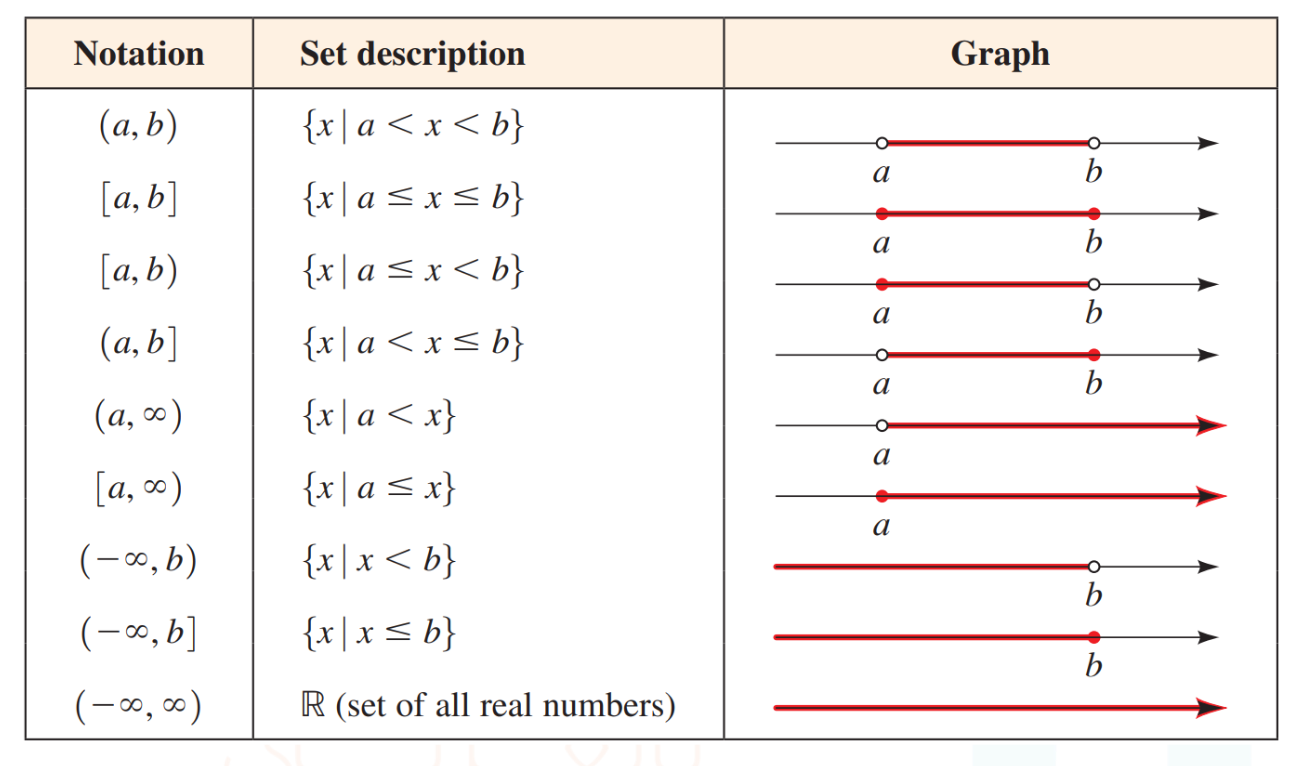
\includegraphics[keepaspectratio]{fig/fig9.png}}

\begin{example}
\protect\hypertarget{exm:unnamed-chunk-119}{}\label{exm:unnamed-chunk-119}

Write Down a Set

\begin{enumerate}
\def\labelenumi{\arabic{enumi}.}
\item
  Set \(A\) such that \(\sup A = \infty\), \(\inf A = 2\):
  \[
  A = [2, \infty)
  \]
\item
  Set \(B\) such that \(\sup B = \infty\), \(\inf B = 1\):
  \[
  B = [1, \infty)
  \]
\item
  Set \(C\) such that \(\sup C = 2\), \(\inf C = -\infty\):
  \[
  C = (-\infty, 2]
  \]
\item
  Set \(D\) such that \(\sup D = \infty\), \(\inf D = -\infty\):
  \[
  D = (-\infty, \infty) = \mathbb{R}
  \]
\end{enumerate}

\end{example}

\chapter{Set Theory}\label{set-theory}

\section{Introduction to Sets}\label{introduction-to-sets}

\begin{definition}
\protect\hypertarget{def:unnamed-chunk-120}{}\label{def:unnamed-chunk-120}

A \textbf{set} is an unordered collection of ``objects.'' The objects in a set are called the \textbf{elements} or \textbf{members} of the set. A set contains its elements.

\begin{itemize}
\tightlist
\item
  A set is usually denoted by a capital letter, say \(A\).
\item
  An element is usually denoted by a lowercase letter, say \(a\) or \(b\).
\item
  We write \(a \in A\) to mean ``\(a\) is an element of \(A\).''
\item
  We write \(a \notin A\) to mean ``\(a\) is not an element of \(A\),'' i.e., \(\sim (a \in A)\).
\end{itemize}

\end{definition}

\begin{example}
\protect\hypertarget{exm:unnamed-chunk-121}{}\label{exm:unnamed-chunk-121}\leavevmode

\begin{itemize}
\item
  Consider the objects \(0, 2, -3, 5\).\\
  The collection \(\{0, 2, -3, 5\}\) is a set.\\
  The elements of this set are \(0, 2, -3, 5\).
\item
  Statement:\\
  \(-3\)is a member of the set \(\{0, 2, -3, 5\}\)
\item
  Statement:\\
  \(4\) is not a member of the set \(\{0, 2, -3, 5\}\)
\end{itemize}

\end{example}

\textbf{Note}

When we consider the collection of all integers, we obtain a set. Any integer is a member of this set. Any object that is not an integer is not a member of this set.

It is not possible to write down all the integers explicitly. However, we can indicate this set using ellipsis notation:

\[
\{\dots, -3, -2, -1, 0, 1, 2, 3, \dots\}
\]

Here, the dots (\(\dots\)) represent the members that are not written down, and it is understood what they are.

\textbf{Set-Builder Notation}

\begin{itemize}
\tightlist
\item
  The set \(\left\{ \frac{1}{2}, \frac{1}{3}, \frac{1}{4}, \dots \right\}\) can be written as: \(\left\{ \frac{1}{n} \mid n \in \mathbb{N} \right\}\)
\end{itemize}

This reads: ``The set whose members are \(\frac{1}{n}\), where \(n\) ranges over all natural numbers.''

\begin{itemize}
\tightlist
\item
  The set \(\{x \mid x \in \mathbb{Z} \text{ and } x > -3\}\) is equal to \(\{-2, -1, 0, 1, 2, 3, 4, \dots\}\)
\end{itemize}

\begin{definition}[Subset]
\protect\hypertarget{def:unnamed-chunk-122}{}\label{def:unnamed-chunk-122}Let \(A\) and \(B\) be sets.\\
We say that \(A\) is a \textbf{subset} of \(B\), denoted \(A \subseteq B\), if and only if every element of \(A\) is also an element of \(B\).

Formally: \(A \subseteq B \iff \forall x \, (x \in A \Rightarrow x \in B)\)
\end{definition}

\begin{example}
\protect\hypertarget{exm:unnamed-chunk-123}{}\label{exm:unnamed-chunk-123}Let \(A = \{1, 2, 4\}\) and \(B = \{1, 2, 3, 4\}\).\\
Then \(A \subseteq B\), but \(B \nsubseteq A\).
\end{example}

\textbf{Note}:
Let \(A\) be a set.\\
Then \(A = \{x \mid p(x)\}\), where \(p(x)\) is a predicate.\\
An element \(x \in A\) if and only if \(p(x)\) is true.

\begin{definition}[Proper Subset]
\protect\hypertarget{def:unnamed-chunk-124}{}\label{def:unnamed-chunk-124}Let \(A\) and \(B\) be sets.\\
We say that \(A\) is a \textbf{proper subset} of \(B\), denoted \(A \subset B\), if and only if:

\begin{enumerate}
\def\labelenumi{\arabic{enumi}.}
\tightlist
\item
  \(A \subseteq B\), and\\
\item
  There exists an element \(x_0 \in B\) such that \(x_0 \notin A\).
\end{enumerate}

Formally:
\[
A \subset B \iff \left( \forall x \, (x \in A \Rightarrow x \in B) \right) \land \left( \exists x_0 \in B \, (x_0 \notin A) \right)
\]
\end{definition}

\begin{definition}[Equality of Sets]
\protect\hypertarget{def:unnamed-chunk-125}{}\label{def:unnamed-chunk-125}Two sets \(A\) and \(B\) are \textbf{equal}, denoted \(A = B\), if and only if:

\begin{enumerate}
\def\labelenumi{\arabic{enumi}.}
\tightlist
\item
  \(A \subseteq B\), and\\
\item
  \(B \subseteq A\)
\end{enumerate}

This is equivalent to:
\[
A = B \iff \forall x \, (x \in A \Leftrightarrow x \in B)
\]
or
\[
A = B \iff \left( \forall x \, (x \in A \Rightarrow x \in B) \right) \land \left( \forall x \, (x \in B \Rightarrow x \in A) \right)
\]
\end{definition}

\begin{definition}[Singleton Set]
\protect\hypertarget{def:unnamed-chunk-126}{}\label{def:unnamed-chunk-126}A set containing exactly one element is called a \textbf{singleton set}.
\end{definition}

\begin{definition}[Empty Set]
\protect\hypertarget{def:unnamed-chunk-127}{}\label{def:unnamed-chunk-127}The set with no elements is called the \textbf{empty set}, denoted by \(\emptyset\) or \(\{\}\).\\
Note: \(\{\emptyset\}\) is not the empty set---it is the set containing the empty set as an element.
\end{definition}

\begin{example}
\protect\hypertarget{exm:unnamed-chunk-128}{}\label{exm:unnamed-chunk-128}\leavevmode

\begin{itemize}
\tightlist
\item
  \(\{x \mid x \in \mathbb{Z} \text{ and } x^2 = 2\} = \emptyset\)
\item
  \(\{x \mid x \in \mathbb{R} \text{ and } x^2 < 0\} = \emptyset\)
\end{itemize}

Observe:
\[
\{x \mid x \in \mathbb{Z} \text{ and } x^2 = 2\} = \{x \mid x \in \mathbb{R} \text{ and } x^2 < 0\}
\]

\end{example}

\begin{definition}[Power Set]
\protect\hypertarget{def:unnamed-chunk-129}{}\label{def:unnamed-chunk-129}Let \(A\) be a set.\\
The \textbf{power set} of \(A\), denoted \(\mathcal{P}(A)\), is defined as:
\[
\mathcal{P}(A) = \{X \mid X \subseteq A\}
\]
That is, the set of all subsets of \(A\).
\end{definition}

\begin{example}
\protect\hypertarget{exm:unnamed-chunk-130}{}\label{exm:unnamed-chunk-130}Let \(A = \{0, 1\}\).\\
Then:
\[
\mathcal{P}(A) = \{\emptyset, \{0\}, \{1\}, \{0, 1\}\}
\]
\end{example}

\begin{definition}[Universal Set]
\protect\hypertarget{def:unnamed-chunk-131}{}\label{def:unnamed-chunk-131}

A \textbf{universal set} is the largest set under consideration, relative to a given context. It contains all elements of the sets being discussed.

\begin{itemize}
\tightlist
\item
  Denoted by \(U\) or \(E\)
\item
  Example: If we are considering subsets of \(\mathbb{R}\), then the universal set is \(\mathbb{R}\)
\end{itemize}

\end{definition}

\textbf{Summary}:

\begin{enumerate}
\def\labelenumi{\arabic{enumi}.}
\item
  \textbf{Subset Definition}\\
  \[
  A \subseteq B \iff \forall x \, (x \in A \Rightarrow x \in B)
  \]
\item
  \textbf{Non-subset}\\
  \[
  A \nsubseteq B \iff \sim (A \subseteq B)
  \]
\item
  \textbf{Equality of Sets}\\
  \[
  A = B \iff A \subseteq B \land B \subseteq A
  \]
\item
  \textbf{Singleton Set}\\
  Example: \(A = \{2\}\)
\item
  \textbf{Empty Set}\\
  \[   \emptyset,\{\}   \]
\item
  \textbf{Power Set}\\
  \[
  \mathcal{P}(A) = \{X \mid X \subseteq A\}
  \]
\item
  \textbf{Universal Set}\\
  Denoted \(E\) or \(U\)
\end{enumerate}

\subsubsection{Set Opertaions}\label{set-opertaions}

\paragraph{Union}\label{union}

Let \(A\) and \(B\) be sets.\\
The \textbf{union} of \(A\) and \(B\), denoted \(A \cup B\), is the set containing all elements that are in \(A\), in \(B\), or in both.

\[
A \cup B = \{ x \mid x \in A \lor x \in B \}
\]

\textbf{Note:}\\
\[
x \in A \cup B \iff x \in A \lor x \in B
\]

\begin{center}\rule{0.5\linewidth}{0.5pt}\end{center}

\paragraph{Intersection}\label{intersection}

Let \(A\) and \(B\) be sets.\\
The \textbf{intersection} of \(A\) and \(B\), denoted \(A \cap B\), is the set containing all elements that are in both \(A\) and \(B\).

\[
A \cap B = \{ x \mid x \in A \land x \in B \}
\]

\textbf{Note:}\\
\[
x \in A \cap B \iff x \in A \land x \in B
\]

\begin{center}\rule{0.5\linewidth}{0.5pt}\end{center}

\paragraph{Complement}\label{complement}

Let \(A \subseteq E\), where \(E\) is a universal set.\\
The \textbf{complement} of \(A\), denoted \(A^c\), is the set of all elements in \(E\) that are not in \(A\).

\[
A^c = \{ x \mid x \in E \land x \notin A \}
\]

\textbf{Note:}\\
\[
x \in A^c \iff x \in E \land x \notin A
\]

\begin{center}\rule{0.5\linewidth}{0.5pt}\end{center}

\paragraph{\texorpdfstring{\textbf{Difference}}{Difference}}\label{difference}

Let \(A\) and \(B\) be sets.\\
The \textbf{difference} of \(A\) and \(B\), denoted \(A \setminus B\), is the set of elements that are in \(A\) but not in \(B\).

\[
A \setminus B = \{ x \mid x \in A \land x \notin B \}
\]

\textbf{Note:}\\
\[
x \in A \setminus B \iff x \in A \land x \notin B
\]

Also called:

\begin{itemize}
\tightlist
\item
  The \textbf{complement of \(B\) in \(A\)}
\item
  The \textbf{relative complement of \(B\) with respect to \(A\)}
\end{itemize}

\chapter{Exercises}\label{exercises-1}

\begin{exercise}
\protect\hypertarget{exr:unnamed-chunk-132}{}\label{exr:unnamed-chunk-132}

Without changing their meanings, convert each of the following sentences into a
sentence having the form ``P if and only if Q.''

\begin{enumerate}
\def\labelenumi{\arabic{enumi}.}
\tightlist
\item
  A series converges whenever it converges absolutely.\\
\item
  For a function to be continuous, it is sufficient that it is differentiable.
\item
  For a function to be continuous, it is necessary that it is integrable.\\
\item
  A function is rational if it is a polynomial.\\
\item
  An integer is divisible by 8 only if it is divisible by 4.
\item
  For matrix \(A\) to be invertible, it is necessary and sufficient that \(\det(A) \neq 0\).\\
\item
  If a function has a constant derivative then it is linear, and conversely.\\
\item
  If \(xy = 0\) then \(x = 0\) or \(y = 0\), and conversely.\\
\item
  If \(a \in \mathbb{Q}\) then \(5a \in \mathbb{Q}\), and if \(5a \in \mathbb{Q}\) then \(a \in \mathbb{Q}\).
\end{enumerate}

\end{exercise}

\begin{exercise}
\protect\hypertarget{exr:unnamed-chunk-133}{}\label{exr:unnamed-chunk-133}

Write truth tables for the following:

\begin{enumerate}
\def\labelenumi{(\roman{enumi})}
\tightlist
\item
  \(p \lor (q \Rightarrow r)\)\\
\item
  \((q \lor r) \Leftrightarrow (r \lor q)\)\\
\item
  \(\sim(\sim p \lor q)\)\\
\item
  \(\sim(p \lor q) \lor (\sim p)\)\\
\item
  \(p \lor (q \land \sim r)\)
\end{enumerate}

\end{exercise}

\begin{exercise}
\protect\hypertarget{exr:unnamed-chunk-134}{}\label{exr:unnamed-chunk-134}Suppose \(p\) is false and\\
\((r \Rightarrow s) \Leftrightarrow (p \land q)\) is true.\\
Find the truth values of \(r\) and \(s\).
\end{exercise}

\begin{exercise}
\protect\hypertarget{exr:unnamed-chunk-135}{}\label{exr:unnamed-chunk-135}

Decide whether the following pairs are logically equivalent:

\begin{enumerate}
\def\labelenumi{(\roman{enumi})}
\tightlist
\item
  \(p \land q\) and \(\sim(\sim p \lor \sim q)\)\\
\item
  \((p \Rightarrow q) \lor r\) and \(\sim((p \land \sim q) \land \sim r)\)\\
\item
  \(p \land (q \lor \sim q)\) and \((\sim p) \Rightarrow (q \land \sim q)\)\\
\item
  \(\sim(p \Rightarrow q)\) and \(p \land \sim q\)\\
\item
  \((p \Rightarrow q) \lor r\) and \(\sim((p \land \sim q) \land \sim r)\)
\end{enumerate}

\end{exercise}

\begin{exercise}
\protect\hypertarget{exr:unnamed-chunk-136}{}\label{exr:unnamed-chunk-136}

Write down the negation of the following statements.

\begin{enumerate}
\def\labelenumi{(\roman{enumi})}
\tightlist
\item
  It's not true that the number 2 is even.\\
\item
  The number 2 is even or the number 3 is odd.\\
\item
  The discriminant is negative only if the quadratic equation has no real solutions.\\
\item
  If a function has a constant derivative then it is linear, and conversely.\\
\item
  Either you pay your tuition or you will be withdrawn from the institute.
\end{enumerate}

\end{exercise}

\begin{exercise}
\protect\hypertarget{exr:unnamed-chunk-137}{}\label{exr:unnamed-chunk-137}Let \(p, q\) and \(r\) be propositions. Let \(T\) denote a tautology.

\begin{enumerate}
\def\labelenumi{(\roman{enumi})}
\tightlist
\item
  Prove the following equivalences:
\end{enumerate}

\begin{itemize}
\tightlist
\item
  \(p \land q \equiv q \land p\)
\item
  \(\neg p \land q \equiv \neg (q \land \neg p)\)
\item
  \(p \land T \equiv T\)
\item
  \(p \lor \neg p \equiv T\)
\item
  \(p \land (q \lor r) \equiv (p \land q) \lor (p \land r)\)
\end{itemize}

\begin{enumerate}
\def\labelenumi{(\roman{enumi})}
\setcounter{enumi}{1}
\tightlist
\item
  Using results in part (i), show that:
\end{enumerate}

\[
[(\neg r) \land p \land q] \lor [(\neg r) \land (\neg p) \land q] \equiv \neg (q \Rightarrow r)
\]
\end{exercise}

\begin{exercise}
\protect\hypertarget{exr:unnamed-chunk-138}{}\label{exr:unnamed-chunk-138}

Consider the statement:\\
``For all integers \(n\), if \(n\) is a multiple of 6 then \(n\) is even.''

Let:

\begin{itemize}
\tightlist
\item
  \(P(n)\): \(n\) is a multiple of 6\\
\item
  \(Q(n)\): \(n\) is even\\
\item
  \(\mathbb{Z}\): the set of all integers
\end{itemize}

\begin{enumerate}
\def\labelenumi{(\roman{enumi})}
\tightlist
\item
  Express the statement in symbolic form.\\
\item
  Write the converse, inverse, and contrapositive in English.\\
\item
  Express the statement using a necessary condition.\\
\item
  Express the statement using a sufficient condition.\\
\item
  Express the statement using ``only if''.
\end{enumerate}

\end{exercise}

\begin{exercise}
\protect\hypertarget{exr:unnamed-chunk-139}{}\label{exr:unnamed-chunk-139}\leavevmode

\begin{enumerate}
\def\labelenumi{(\roman{enumi})}
\tightlist
\item
  What is the English interpretation of the contrapositive of:
\end{enumerate}

\[
\forall \epsilon > 0 \, \forall x \in D(f) \, \exists \delta > 0, \quad |f(x) - l| < \epsilon \Rightarrow |x - a| \geq \delta
\]

\begin{enumerate}
\def\labelenumi{(\roman{enumi})}
\setcounter{enumi}{1}
\tightlist
\item
  What is the English interpretation of the negation of:
\end{enumerate}

\[
\exists \delta > 0 \, \forall x \in S, \quad S \cap N^c(a, \delta) = \emptyset
\]

\end{exercise}

\begin{exercise}
\protect\hypertarget{exr:unnamed-chunk-140}{}\label{exr:unnamed-chunk-140}

Consider the following argument for an integer \(n\):

\begin{itemize}
\tightlist
\item
  \(n\) is odd.\\
\item
  If \(n\) is not odd, then \(n^2\) is not odd.\\
\item
  Therefore, \(n^2\) is even.
\end{itemize}

Let:

\begin{itemize}
\tightlist
\item
  \(p\): \(n\) is odd\\
\item
  \(q\): \(n^2\) is odd
\end{itemize}

\begin{enumerate}
\def\labelenumi{(\roman{enumi})}
\tightlist
\item
  Express the argument symbolically.\\
\item
  Determine whether the argument is valid.
\end{enumerate}

\end{exercise}

\begin{exercise}
\protect\hypertarget{exr:unnamed-chunk-141}{}\label{exr:unnamed-chunk-141}

Prove each of the following statements:

\begin{itemize}
\tightlist
\item
  \begin{enumerate}
  \def\labelenumi{(\alph{enumi})}
  \tightlist
  \item
    For all integers \(a\), \(b\), and \(c\) with \(a \neq 0\), if \(a \mid b\) and \(a \mid c\), then \(a \mid (b - c)\).
  \end{enumerate}
\item
  \begin{enumerate}
  \def\labelenumi{(\alph{enumi})}
  \setcounter{enumi}{1}
  \tightlist
  \item
    For each \(n \in \mathbb{Z}\), if \(n\) is an odd integer, then \(n^3\) is an odd integer.
  \end{enumerate}
\item
  \begin{enumerate}
  \def\labelenumi{(\alph{enumi})}
  \setcounter{enumi}{2}
  \tightlist
  \item
    For each integer \(a\), if \(4 \mid (a - 1)\), then \(4 \mid (a^2 - 1)\).
  \end{enumerate}
\end{itemize}

\end{exercise}

\begin{exercise}
\protect\hypertarget{exr:unnamed-chunk-142}{}\label{exr:unnamed-chunk-142}

Let \(n\) be an integer. Prove each of the following:

\begin{itemize}
\tightlist
\item
  \begin{enumerate}
  \def\labelenumi{(\alph{enumi})}
  \tightlist
  \item
    If \(n\) is even, then \(n^3\) is even.
  \end{enumerate}
\item
  \begin{enumerate}
  \def\labelenumi{(\alph{enumi})}
  \setcounter{enumi}{1}
  \tightlist
  \item
    If \(n^3\) is even, then \(n\) is even.
  \end{enumerate}
\item
  \begin{enumerate}
  \def\labelenumi{(\alph{enumi})}
  \setcounter{enumi}{2}
  \tightlist
  \item
    The integer \(n\) is even if and only if \(n^3\) is even.
  \end{enumerate}
\item
  \begin{enumerate}
  \def\labelenumi{(\alph{enumi})}
  \setcounter{enumi}{3}
  \tightlist
  \item
    The integer \(n\) is odd if and only if \(n^3\) is odd.
  \end{enumerate}
\end{itemize}

\end{exercise}

\begin{exercise}
\protect\hypertarget{exr:unnamed-chunk-143}{}\label{exr:unnamed-chunk-143}\leavevmode

\begin{itemize}
\tightlist
\item
  \begin{enumerate}
  \def\labelenumi{(\alph{enumi})}
  \tightlist
  \item
    Write the contrapositive of the following statement:\\
    \emph{For all positive real numbers \(a\) and \(b\), if \(\sqrt{ab} \neq \frac{a + b}{2}\), then \(a \neq b\).}
  \end{enumerate}
\item
  \begin{enumerate}
  \def\labelenumi{(\alph{enumi})}
  \setcounter{enumi}{1}
  \tightlist
  \item
    Is this statement true or false?\\
    Prove the statement if it is true or provide a counterexample if it is false.
  \end{enumerate}
\end{itemize}

\end{exercise}

\begin{exercise}
\protect\hypertarget{exr:unnamed-chunk-144}{}\label{exr:unnamed-chunk-144}Is the following proposition true or false?

\begin{quote}
For all integers \(a\) and \(b\), if \(ab\) is even, then \(a\) is even or \(b\) is even.
\end{quote}

Justify your conclusion by writing a proof if the proposition is true or by providing a counterexample if it is false.
\end{exercise}

\begin{exercise}
\protect\hypertarget{exr:unnamed-chunk-145}{}\label{exr:unnamed-chunk-145}

Are the following propositions true or false? Justify your conclusion.

\begin{itemize}
\tightlist
\item
  \begin{enumerate}
  \def\labelenumi{(\alph{enumi})}
  \tightlist
  \item
    There exist integers \(x\) and \(y\) such that \(4x + 6y = 2\).
  \end{enumerate}
\item
  \begin{enumerate}
  \def\labelenumi{(\alph{enumi})}
  \setcounter{enumi}{1}
  \tightlist
  \item
    There exist integers \(x\) and \(y\) such that \(6x + 15y = 2\).
  \end{enumerate}
\item
  \begin{enumerate}
  \def\labelenumi{(\alph{enumi})}
  \setcounter{enumi}{2}
  \tightlist
  \item
    There exist integers \(x\) and \(y\) such that \(6x + 15y = 9\).
  \end{enumerate}
\end{itemize}

\end{exercise}

  \bibliography{book.bib,packages.bib}

\end{document}
